\documentclass[12pt]{article}
\usepackage{amsmath, amssymb, graphicx, natbib, geometry}
\geometry{margin=1in}
\usepackage{setspace}
\usepackage{titlesec}
\usepackage{booktabs}
\usepackage{hyperref}
\hypersetup{hidelinks} % plain black links, no colored boxes
\usepackage{float}
\usepackage{xcolor}
\usepackage[most]{tcolorbox}
\usepackage{tikz}
\usetikzlibrary{positioning, shapes.geometric, arrows.meta, calc}
\usepackage{pgfplots}
\pgfplotsset{compat=1.17}
\usepackage{tabularx}
\usepackage{array}
\newcolumntype{L}[1]{>{\raggedright\arraybackslash}p{#1}} % ragged-right text columns for all tables
\usepackage{mdframed}
\usepackage[table]{xcolor}
\usepackage{natbib}

% Unified styling for all Definition / Proposition / Remark boxes (R1, comment 2)
\tcbset{
  enhanced,
  colback=white,
  colframe=black!70,
  boxrule=0.6pt,
  arc=1pt,
  left=6pt, right=6pt, top=4pt, bottom=4pt,
  fonttitle=\bfseries\small,
  coltitle=black,
  colbacktitle=gray!12,
  titlerule=0.4pt,
  before skip=10pt, after skip=10pt
}


\title{Economic Scarcity as Value: A Universal Framework for Blockchain and Beyond}
\author{Agisilaos Papadogiannis\thanks{
Independent Researcher (PhD, MBA). \textit{Correspondence:} apapadogiannis@gmail.com. \textit{ORCID:} 0009-0002-7753-7052. Data, code and replication files: \url{https://github.com/apapadogiannis/economic-scarcity-as-value}, archived at \url{https://doi.org/10.5281/zenodo.24051776}.
}}

\begin{document}

\maketitle

\begin{abstract}
Classical finance values assets as discounted expected cash flows, taking for granted the structural conditions that make those flows possible. This paper advances an alternative principle: \emph{economic scarcity}, the monetizable intersection of desirability and constrained access, as the foundation of value, with blockchain networks as a uniquely transparent setting in which scarcity and incentives are encoded directly in protocol design. We develop a structural valuation framework that links five value elements, Purpose, Incentives, Consensus, Tokenomics, and Network Effects, to both economic scarcity and the architectural layers of distributed systems, and formalize it into a general network value function. An illustrative case study of Bitcoin, Ethereum, and Bittensor shows how the framework separates the share of a network's valuation explained by its measurable structure from the share that rests on expectations.
\end{abstract}

\vspace{1em}
\noindent\textbf{Keywords:} Economic scarcity, Blockchain valuation, Network architecture, Tokenomics, Distributed systems, Network effects, Consensus mechanisms, Proof-of-Work (PoW), Proof-of-Stake (PoS), Yuma Consensus, Bittensor, Asset pricing



%%%%%%%%%%%%%%%%%%%%%%%%%%%%%%%%%%%%%%%%%%%%%%%%%%%%%%%%%%%%%%%%%%%%%%%%%
\section{Introduction}

What gives an asset economic value? In classical finance, value is treated as a discounted sum of expected cash flows \citep{williams1938theory, damodaran2012investment}, assuming that monetizable outcomes already exist and that markets merely price them. This perspective bypasses a foundational question: \textit{what enables those cash flows to arise in the first place?} We propose that value originates from \emph{economic scarcity}, defined as the monetizable intersection of \textbf{desirability} and \textbf{physical scarcity} (constrained access). This principle is universal, applying to asset classes as varied as equities, natural resources, and collectibles, as well as to digital tokens. It has deep historical roots in the marginalist tradition of value theory, where both utility and scarcity are necessary for economic valuation \citep{jevons1871political, menger1871principles}, and it aligns with insights from behavioral finance \citep{barberis1998investor, hong2007disagreement}, institutional theory \citep{merton1987simple, pagano1998choice}, and cultural economics \citep{lin2025culture}.

While economic scarcity applies broadly, blockchain networks offer the most tractable and transparent environment in which to study it. Their core components, such as protocol functionality, supply discipline, and user adoption, are structurally embedded and publicly observable on-chain. Unlike traditional firms that rely on legal enforcement and centralized administration, blockchains implement scarcity and incentive mechanisms directly through code and consensus protocols \citep{cong2019blockchain, cong2021tokenomics}. This architecture enables real-time visibility into both the supply schedule and user behavior, providing a unique laboratory for observing how economic scarcity can give rise to value even in the absence of conventional revenue streams \citep{nadler2020fair, urquhart2023future}.

The five structural elements developed in this paper, namely Purpose, Incentives, Consensus, Tokenomics, and Network Effects, are both economic drivers in the proposed valuation framework and fundamental components of blockchain network architecture. Each corresponds to a distinct design layer: functional specification (Purpose), incentive mechanism design (Incentives), trust and state synchronization (Consensus), monetary and resource allocation rules (Tokenomics), and emergent interaction topology (Network Effects) \citep{gans2019economics, catalini2020some, saleh2021blockchain, cong2021tokenomics}. By linking these architectural primitives to the economic scarcity framework, we build an explicit bridge between protocol engineering and asset valuation, showing how design choices in distributed systems translate into measurable scarcity conditions and monetizable value \citep{huberman2021monetizing, urquhart2023future, rao2023bittensor}.


\subsection{Prior Literature}

Existing blockchain valuation approaches fall into four main categories. First, cost-of-production models, such as the one proposed by \citet{hayes2015cost}, estimate cryptocurrency value based on marginal mining costs and energy input. Second, empirical network models rely on user adoption metrics, often approximated by Metcalfe’s Law or its variants, as discussed by \citet{GandalHalaburda2016}, \citet{Peterson2018}, and \citet{cong2019blockchain}. Third, tokenomics-based studies examine how token design parameters influence valuation, including issuance schedules, governance mechanisms, and incentive structures, as analyzed by \citet{cong2021tokenomics}, \citet{huberman2021monetizing}, and \citet{catalini2020some}. Finally, market-based econometric models investigate behavioral dynamics, return predictability, and risk premia. For instance, \citet{LiuTsyvinski2022} study cryptocurrency factor exposures using an empirical asset pricing model, while \citet{urquhart2022ethereum} explore time-varying volatility and return spillovers.

In addition, several studies employ statistical and machine learning tools to forecast prices or detect inefficiencies. \citet{Kristoufek2015} apply wavelet coherence to analyze Bitcoin price drivers across time and frequency domains. \citet{Koutmos2018} uses Vector Autoregressive (VAR) analysis to show that Bitcoin transaction activity temporarily predicts returns. \citet{dinizmaganini2021bitcoin} evaluate the safe haven properties of Bitcoin during the COVID-19 pandemic and assess price efficiency. \citet{bouteska2024cryptocurrency} provide a comparative analysis of cryptocurrency forecasting using ensemble and deep learning methods. In addition to this, \citet{nadler2020fair} directly address token valuation, showing that crypto assets are priced through endogenous mechanisms that reflect both speculative activity and protocol utility.

Beyond blockchain-specific literature, existing valuation models for digital platforms\footnote{Digital platforms are infrastructures that facilitate user interactions and enable value creation through complementary assets such as third-party apps, services, or content.} emphasize user growth, pricing strategy, and cross-side externalities. In two-sided market frameworks, platform value is often modeled as a function of adoption on each side, alongside the strength of network effects \citep{rochet2003platform, evans2003platform, parker2016platform}.\footnote{A two-sided market is a platform-based structure in which two distinct participant groups interact through a common intermediary, and the value to one group depends on the size or engagement of the other. Examples include credit card networks (merchants and cardholders), marketplaces (buyers and sellers), and app stores (developers and users). The platform designs pricing and access strategies to coordinate both sides, often subsidizing one to attract the other and maximize interaction volume.} Practitioners frequently apply heuristics such as average revenue per user (ARPU) multiplied by monthly active users, implicitly assuming monetization scales linearly with adoption. However, these approaches capture interaction-driven growth without formalizing the structural preconditions necessary for value creation. In particular, existing platform valuation theories typically lack an explicit economic theory of scarcity.

Despite these varied contributions, the existing literature does not offer a structurally unified valuation framework based on the concept of economic scarcity, which we define as the monetizable intersection of desirability and constrained access (physical scarcity). The closest antecedent is the dynamic tokenomics literature: Cong, Li, and Wang \citep{cong2021tokenomics} jointly endogenize user adoption, transactional demand, network externalities, and token price in a dynamic equilibrium model, and Cong and He \citep{cong2019blockchain} analyze how blockchain-enabled contracting shapes value creation. Our contribution is complementary rather than competing: instead of modeling the dynamics of adoption and price, we provide a \emph{structural decomposition} of the scarcity preconditions of value, five architectural elements and their mapping onto desirability and physical scarcity, together with an attribution method that measures how much of an observed valuation these structural components explain. To our knowledge, no existing framework has formally positioned economic scarcity, defined through the combined effects of desirability and constrained access, as the foundational determinant of monetizable value across asset classes. In the context of blockchain networks, these scarcity drivers are inseparable from the underlying network architecture, linking economic outcomes directly to technological design.

\subsection{Contributions}

Our paper makes three contributions to the literature on valuation, network architecture, and economic theory:

\begin{itemize}
    \item \textbf{Definition of Economic Scarcity as Value:} We define \emph{economic scarcity} as the monetizable intersection of desirability and constrained access (Section~\ref{sec:scarcity_def}), and formalize it in an axiomatically motivated valuation form. This concept shifts the basis of valuation from cash flow projections to the structural preconditions of value.

    \item \textbf{An Architecture--Valuation Bridge:} We introduce five foundational elements, Purpose, Incentives, Consensus, Tokenomics, and Network Effects, that determine a blockchain protocol's capacity to generate economic value (Section~\ref{sec:framework_elements}). Each element maps directly to a core architectural layer in distributed system design, making explicit how protocol engineering choices shape the conditions for economic scarcity. The native token is characterized as the monetization interface that binds these elements together (Section~\ref{sec:native_token}), and Appendix~\ref{appendix:tokens_vs_equity} anchors the mapping by contrasting tokens with common equity.

    \item \textbf{An Implied-Desirability Attribution Method with a Comparative Case Study:} We propose a structural valuation model integrating protocol design, scarcity constraints, and user adoption (Section~\ref{sec:valuation_framework}), in which desirability is recovered as an \emph{implied} residual under an explicitly disclosed measurement convention. We illustrate the method on Bitcoin, Ethereum, and Bittensor.
\end{itemize}

%%%%%%%%%%%%%%%%%%%%%%%%%%%%%%%%%%%%%%%%
\section{Economic Scarcity as the Foundation of Value}
\label{sec:scarcity_def}

Scarcity is a foundational concept in both economics and finance, yet its meaning and its implications for valuation vary by context. Not all forms of scarcity generate value. Some goods are objectively rare but economically irrelevant. Others are abundant but highly sought after. To build a coherent theory of asset valuation, we must first clarify what kind of scarcity is relevant for monetizable outcomes.

\subsection{Physical vs. Economic Scarcity}

We begin by distinguishing between physical scarcity, which refers to constrained supply, and economic scarcity, which arises when such constraints apply to something that is also desired.

\begin{tcolorbox}[title=\textbf{Definition (Physical Scarcity)}]
Physical scarcity refers to a condition in which a good, asset, or service is objectively limited in quantity or availability, regardless of whether it is valued or monetized.
\end{tcolorbox}

A physically scarce item is not necessarily valuable. A material may be rare but unused; a token may be capped but unwanted. Without accompanying demand, physical limitation alone does not imply market value.

\begin{tcolorbox}[title=\textbf{Definition (Economic Scarcity)}]
Economic scarcity refers to a condition in which access to a desirable good, service, or functionality is constrained in a way that enables monetization through exchange, yield, or resale.

In essence, economic scarcity arises from the combination of \textit{physical scarcity} (constrained access) and \textit{desirability} (perceived value).
\end{tcolorbox}


This distinction echoes classical views from the marginalist tradition in economics, where value arises not simply from rarity but from the interplay between scarcity and subjective utility \citep{menger1871principles, jevons1871political}. Economic scarcity captures this duality, emphasizing that value only emerges when constrained access meets desirability.
%--------------------------------------
\subsection{Economic Scarcity as Value}

Classical finance treats value as a discounted sum of expected cash flows \citep{williams1938theory, brealey2022principles, damodaran2012investment}. This framework presumes that monetizable outcomes already exist, and that markets merely price them. However, this view bypasses a foundational question: \textit{what enables those cash flows to arise in the first place?}


We propose a more foundational perspective: that \textbf{economic scarcity is the upstream condition that enables value to exist}. Before a cash flow can be priced, it must first be created. That creation is only possible when access to something desirable is constrained in a way that allows monetization through resale, yield, or exclusivity.

\begin{tcolorbox}[title=\textbf{Proposition 1}]
Economic scarcity is the upstream determinant of monetizable value. That is,
\begin{equation}
\text{Value}_t \approx \text{Economic Scarcity}_t.
\end{equation}
\end{tcolorbox}

This idea echoes foundational work in marginalist economics, where value emerges not from intrinsic properties but from the interaction between subjective utility and constrained supply \citep{menger1871principles, jevons1871political}. In modern microeconomic theory, price reflects marginal willingness to pay under scarcity constraints rather than inherent worth \citep{varian1992microeconomic}. Scarcity should therefore be seen not as a residual modifier of value but as its structural basis.

In traditional finance, scarcity at the asset level often reflects a deeper form of economic scarcity embedded in the underlying business model, product, or service. Financial instruments rarely embody scarcity on their own. Instead, they derive value from structural constraints elsewhere in the system \citep{tirole1988theory, porter1985competitive, demsetz1973industry}.

For example:
\begin{itemize}
    \item \textbf{Equity value} is ultimately driven by the scarcity of the firm’s product or service offering, typically achieved through \textit{product differentiation} or \textit{cost leadership}, which create competitive advantages and pricing power \citep{porter1985competitive};

    \item \textbf{Patents and intellectual property rights} restrict imitation and protect future cash flows linked to unique products or technologies \citep{shapiro1985licensing, gallini2002intellectual};

    \item \textbf{Licensing agreements and exclusivity clauses} limit access to distribution channels or geographic markets \citep{caves1983contractual, jaffe1993geographic};

    \item \textbf{Regulatory barriers and legal protections} prevent competitive entry, sustaining rents in capital-intensive or heavily regulated sectors \citep{demsetz1973industry, stigler1971regulation};

    \item \textbf{Share buybacks and limited public float} maintain equity scarcity in secondary markets, reflecting underlying competitive advantages or investor demand \citep{pontiff2006liquidity}.
\end{itemize}

In each case, the scarcity of the financial asset is meaningful only because it maps to a real constraint on access, production, or differentiation at the economic level.

These mechanisms do not generate cash flows on their own. Instead, they create the structural conditions under which monetizable outcomes, such as profits, royalties, or resale rights, can emerge. In this sense, scarcity is a prerequisite for value, not a secondary attribute.

In decentralized systems, physical scarcity is deliberately engineered through protocol rules such as token supply caps, validator quotas, and block size limits. These constraints are hard-coded but do not create value by themselves. Scarcity becomes economically meaningful only when there is user demand for the constrained resource. When protocol-enforced limits align with perceived utility and growing adoption, they generate economic scarcity, enabling value capture without traditional cash flows. Monetization can occur through token price appreciation \citep{hayes2015cost}, transaction-based access \citep{lu2025unveiling}, or native mechanisms like staking rewards and fee distribution \citep{saleh2021blockchain, ramachandran2021defi}. As Cong and He show, such endogenous value arises when economic logic is embedded into the system's architecture \citep{cong2019blockchain}.



Digitally enforced scarcity has emerged as a primary source of value in many decentralized systems, including NFTs and tokenized assets, where monetization often occurs without reference to traditional income streams \citep{lu2025unveiling}. Our framework formalizes this perspective by treating economic scarcity, defined through desirability and constrained access, as the structural foundation of value. This approach applies across asset classes and valuation regimes. Rather than viewing scarcity as a residual feature or external assumption, we treat it as the condition that makes monetizable outcomes possible in the first place.

%--------------------------------------
\subsection{Defining Economic Scarcity}

Economic scarcity is not a binary state but a structural condition arising from the interplay of two foundational elements:
\begin{itemize}
  \item \textbf{Desirability} (\( D_t \)): a demand-side attribute reflecting perceived usefulness, cultural or strategic relevance, and utility;
  \item \textbf{Physical Scarcity} (\( S_t \)): a supply-side attribute capturing limits in issuance, availability, or access.
\end{itemize}

This dual structure echoes classical marginalist economics, where value emerges from the interaction between subjective utility and constrained supply \citep{menger1871principles, jevons1871political}.

We now formalize this idea:

\begin{tcolorbox}[title=\textbf{Proposition 2}]
Economic scarcity arises when physical scarcity and desirability are jointly present and mutually reinforcing. Formally:
\begin{equation}
\text{Economic Scarcity}_t := D_t \cdot S_t \cdot F(D_t, S_t),
\label{eq:economic_scarcity}
\end{equation}
where:
\begin{itemize}
  \item \( D_t \): Desirability at time \( t \),
  \item \( S_t \): Physical scarcity at time \( t \),
  \item \( F(D_t, S_t) \): a continuously differentiable interaction function satisfying
  \[
  \frac{\partial F}{\partial D_t} > 0 \quad \text{and} \quad \frac{\partial F}{\partial S_t} > 0.
  \]
\end{itemize}
These conditions define the class of \emph{smooth, strictly complementary} interaction functions to which the analysis applies. Non-smooth alternatives, such as the bottleneck form \( \min(D_t, S_t) \), fall outside this class: they are weakly rather than strictly monotone and non-differentiable where the two inputs coincide. Such forms are catalogued separately in Appendix~\ref{appendix:f_forms}.
\end{tcolorbox}

The multiplicative structure in Equation~\ref{eq:economic_scarcity} ensures that economic scarcity vanishes if either component is absent. A resource that is desirable but not physically scarce, or physically scarce but not desired, cannot command market value. This reflects a structural complementarity between constrained access and perceived relevance.

Moreover, this formulation supports a log-linear interpretation. Taking logarithms yields:
\begin{equation}
\log(\text{Economic Scarcity}_t) = \log D_t + \log S_t + \log F(D_t, S_t),
\label{eq:log_scarcity}
\end{equation}
which decomposes economic scarcity into additive components on a logarithmic scale. This is consistent with common functional forms in economics and finance, such as Cobb–Douglas production functions, constant elasticity demand models, and log-linear valuation frameworks \citep{varian1992microeconomic, campbell1997econometrics}.

The interaction term \( F(D_t, S_t) \) captures how scarcity and desirability reinforce one another. The more constrained a desirable asset, the higher its marginal value; and the more desirable a physically scarce asset, the greater the competition to access it. This feedback loop underlies real-world value dynamics, from housing market bidding wars to the valuation of Bitcoin despite limited transactional capacity \citep{hayes2015cost, conley2021blockchain}.

This interaction is illustrated qualitatively in Table~\ref{tab:interaction_d_s}, which presents the four canonical combinations of desirability and physical scarcity and their implications for economic value.


\begin{table}[H]
\centering
\vspace{-1em} % Reduce space before the table
\caption{Desirability and Physical Scarcity Determining Economic Value}
\label{tab:interaction_d_s}
\renewcommand{\arraystretch}{1.1} % Tighter vertical spacing
\begin{tabular}{@{}L{3.8cm}L{3.8cm}L{7.2cm}@{}}
\toprule
\rowcolor{gray!15}
\textbf{Desirability (\( D_t \))} & \textbf{Physical Scarcity (\( S_t \))} & \textbf{Interpretation} \\
\midrule
\textbf{Low} & \textbf{Low} & Asset lacks both appeal and constraint; generates negligible or zero value. \\
\textbf{Low} & \textbf{High} & Technically limited or rare item with no use case or demand; may appear valuable but lacks liquidity or utility. \\
\textbf{High} & \textbf{Low} & Popular or useful asset that is easily accessible or oversupplied; value potential limited by weak monetization. \\
\textbf{High} & \textbf{High} & Strongly desired and meaningfully constrained asset; optimal conditions for monetizable economic scarcity. \\
\bottomrule
\end{tabular}
\vspace{-0.5em} % Reduce space after the table
\end{table}


\paragraph{Interpretive Note on \( F(D_t, S_t) \).} 
The function \( F(D_t, S_t) \) is deliberately left general, as it reflects how scarcity and desirability reinforce one another in context-dependent ways. In scalable systems, particularly digital platforms and decentralized networks, this interaction is often mediated by user participation. As adoption grows, it can simultaneously enhance perceived utility and intensify competitive access, thereby amplifying both \( D_t \) and \( S_t \). In such settings, network effects offer a tractable and empirically grounded approximation of the interaction term. Specifically, we may write:
\begin{equation}
F(D_t, S_t) \approx u_t^{\alpha},
\label{eq:interaction_approx}
\end{equation}
where \( u_t \) denotes the scale of adoption and \( \alpha \geq 1 \) reflects the strength of interaction effects across the user base, with \( \alpha \in [1, 2.5] \) spanning the regimes considered in this paper. This formulation draws on established theories of network value, such as Metcalfe’s Law \citep{metcalfe1995metcalfe}, Reed’s Law \citep{reed2001law}, and empirical findings on digital platform scaling \citep{evans2003two, rochet2006two, cong2019blockchain}. A broader discussion of alternative specifications for \( F(D_t, S_t) \), including additive, logarithmic, and bottleneck-constrained forms, is provided in Appendix~\ref{appendix:f_forms}. Equation~\ref{eq:interaction_approx} motivates the structural valuation form introduced in the next subsection.

%--------------------------------------
\subsection{Economic Scarcity with Network Effects}

The previous section proposed that economic scarcity arises from the joint presence of desirability and physical scarcity, amplified by an interaction function \( F(D_t, S_t) \). In digitally scalable systems, particularly blockchain networks and platform-based markets, this amplification is often mediated by user adoption. As more users participate in a system, they not only contribute to its economic scale but also increase its perceived utility and exclusivity. Adoption can trigger reinforcing feedback loops that amplify the joint economic impact of desirability and scarcity via the function \( F(D_t, S_t) \), rather than increasing \( D_t \) or \( S_t \) directly. As usage grows, perceived utility rises and competition for constrained resources intensifies.


This phenomenon has been widely documented in network theory and digital economics. In online platforms, larger user bases increase personalization, social proof, and systemic reliability, all of which enhance desirability \citep{zhang2010value, brousseau2007internet}. At the same time, when access is limited, whether by design or protocol constraints, growing participation can intensify scarcity perception. These dynamics justify using network effects as a proxy for the amplification term \( F \), particularly in systems where user-driven value creation is endogenous to the architecture \citep{cong2019blockchain, easley2010networks}.

Substituting \( F(D_t, S_t) \approx u_t^\alpha \) (Equation \ref{eq:interaction_approx}) into the general economic scarcity formulation (Equation \ref{eq:economic_scarcity}) leads to a valuation structure grounded in observable participation metrics.

\begin{tcolorbox}[title=\textbf{Proposition 3 (Valuing Scarcity under Network Effects)}]
Let \( D_t \) denote time-\( t \) desirability, \( S_t \) the corresponding physical scarcity, and \( u_t \) the scale of adoption. Then the asset value at time \( t \) can be expressed as:
\begin{equation}
V_t \approx D_t \cdot S_t \cdot u_t^{\alpha},
\label{eq:structural_valuation}
\end{equation}
where \( \alpha \geq 1 \) captures the intensity of adoption-driven reinforcement (\( \alpha \in [1, 2.5] \) in this paper's analyses).
\end{tcolorbox}

\paragraph{Axiomatic Motivation.}
The structure in Equation~\eqref{eq:structural_valuation} is \emph{consistent with}, though not uniquely determined by, three intuitive conditions; it is a parsimonious member of the admissible class of functional forms catalogued in Appendix~\ref{appendix:f_forms}:
\begin{itemize}
  \item \textbf{Zero Bound:} If either \( D_t = 0 \) or \( S_t = 0 \), then \( V_t = 0 \); value requires both perceived utility and constrained access.
  \item \textbf{Positive Scaling:} For given \( D_t \) and \( S_t \), value increases with adoption. The exponent \( \alpha \geq 1 \) governs this amplification.
  \item \textbf{Amplified Interaction:} The term \( u_t^\alpha \) reflects how adoption both realizes and reinforces value, by amplifying the effect of desirability and scarcity in tandem.
\end{itemize}

This is not a product of independent variables but a structural feedback mechanism: adoption enables the monetization of desirability and scarcity, which in turn attracts further participation. This logic builds on foundational results in network economics. Metcalfe’s Law (\( \alpha = 2 \)) models quadratic user interaction value \citep{metcalfe1995metcalfe}, while Reed’s Law (\( \alpha > 2 \)) allows exponential scaling via group formation \citep{reed2001law}; \citet{briscoe2006metcalfe} argue, conversely, that network value scales only as \( n \log n \). Easley and Kleinberg \citep{easley2010networks} highlight how network topology shapes both reach and resilience of value creation.

In blockchain systems, Cong and He \citep{cong2019blockchain} show that endogenous value arises from feedback between protocol design and user engagement. Equation~\eqref{eq:structural_valuation} extends this insight by modeling value as a co-evolving function of structural scarcity, perceived utility, and adoption-driven amplification.

\paragraph{Interpretive Note.}
It is tempting to distinguish between “per-user value” and “user scale.” However, in systems with dynamic and reflexive adoption, this distinction is artificial. As more users enter the system:
\begin{itemize}
    \item \( D_t \) may appear to rise due to increased visibility, validation, or emergent utility;
    \item \( S_t \) may appear to rise as a fixed supply serves a larger user base, increasing perceived exclusivity;
    \item But such feedback effects are not modeled as changes to \( D_t \) or \( S_t \) directly. Instead, they are captured by the scaling function \( F(D_t, S_t) = u_t^\alpha \), which acts as a proxy for their interaction.
\end{itemize}

In this sense, adoption is not just a third variable but a structural amplifier: it both realizes and intensifies the economic relevance of desirability and scarcity. The term \( u_t^\alpha \) reflects both the scale of participation and the intensity of user-driven reinforcement. This enables value to scale non-linearly, even in the absence of explicit cash flows. \footnote{The multiplicative interaction between \( D_t \), \( S_t \), and \( F(D_t, S_t) \) is conceptually analogous to the joint effect of correlated variables in probability theory, where dependence amplifies outcomes. However, in this framework, the variables are deterministic economic primitives, and \( F \) encodes structural rather than statistical amplification.}

Equation~\eqref{eq:structural_valuation} thus provides a tractable yet general lens for understanding asset value across a wide range of contexts, including, but not limited to, decentralized systems and platform-based environments.




%--------------------------------------
\subsection{Relation to DCF Valuation}

This scarcity-based framework complements discounted cash flow (DCF) models. In earlier work \citep{papadogiannis2025dualrisk}, it was shown that cryptoassets and other unconventional instruments can be valued using generalized DCF models when expectations and discount rates are separated. That framework starts with cash flow projections. The present framework asks the upstream question: \textit{when does monetization arise to begin with?}

Economic scarcity provides that answer. It is not merely an input to valuation, but the structural condition that makes valuation meaningful. While behavioral models of asset pricing \citep{barberis1998investor, daniel1998investor, hong2000bad, benartzi1995myopic, thaler1997effect, papadogiannis2025dualrisk} emphasize how investor sentiment, cognitive biases, and limited attention can drive deviations from fundamental value, our framework addresses a more foundational question: what structural conditions make value emerge at all. In this sense, we complement behavioral perspectives by embedding perceived desirability into the very construction of monetizable fundamentals.


%-------------------------------------------------
\subsection{Beyond Blockchain}

While blockchain networks offer the clearest expression of economic scarcity-driven valuation, due to explicit tokenomics, transparent protocol rules, and observable adoption metrics, the underlying framework is general. Economic scarcity, as the joint outcome of desirability and constrained access, underpins value creation across many asset classes.

In traditional finance, physical \textit{scarcity} may stem from legal protection, institutional friction, or controlled issuance \citep{merton1987simple, pagano1998choice}. \textit{Desirability} may reflect expectations of future cash flows, product differentiation, cost advantage, strategic relevance, or cultural symbolism \citep{barberis1998investor, porter1985competitive, lu2025unveiling}. Adoption scales value when broader participation enhances utility, credibility, or liquidity \citep{rochet2003platform, easley2019from}.



\begin{tcolorbox}[title=\textbf{Applicability to Traditional Assets}]
The economic scarcity framework applies to any asset class where three structural conditions are jointly satisfied:

\begin{itemize}
  \item \textbf{Desirability (\( D_t \))}: Demand is not passive but reflects perceived utility, strategic advantage, or cultural significance. This includes cases where investors or users attribute future potential, brand strength, emotional value, or strategic positioning to the asset.
  
  \item \textbf{Physical Scarcity (\( S_t \))}: Supply is meaningfully constrained, either by design (e.g., fixed token supply), regulation (e.g., licensing or float restrictions), or institutional friction (e.g., barriers to entry, limited issuance mechanisms). These constraints limit access and availability, which is necessary for scarcity to become economically significant.
  
  \item \textbf{Interaction Dynamics (\( F(D_t, S_t) \))}: Adoption or engagement amplifies value through visibility, liquidity, or network reinforcement. When user participation increases, it enhances perceived utility and deepens the salience of access constraints. This feedback mechanism, often modeled via network effects, transforms static scarcity into scalable economic value.
\end{itemize}
\end{tcolorbox}

\vspace{0.5em}

Examples include:

\begin{itemize}
  \item \textbf{Common stocks}: Desirability arises from product differentiation, cost leadership, or strategic positioning that drive firm performance \citep{porter1985competitive}; physical scarcity emerges through float restrictions, insider holdings, or share buybacks \citep{pontiff2006liquidity}; adoption reflects investor base expansion, institutional inclusion, or index exposure \citep{barberis2005comovement}.

  \item \textbf{Digital platforms}: User demand drives engagement; access restrictions or reputation mechanisms create scarcity; adoption fuels feedback loops and network effects \citep{rochet2003platform, parker2016platform}.

  \item \textbf{Collectibles and cultural assets}: Desirability from aesthetic or symbolic value; physical scarcity from uniqueness; adoption through collector interest or social signaling \citep{akerlof2010identity, lin2025culture}.

  \item \textbf{Natural resources}: Scarcity from finite availability; desirability from utility; adoption via industrial or sovereign demand \citep{hotelling1931economics, kilian2009oil}.
\end{itemize}

What distinguishes \textbf{blockchain networks} is that physical scarcity, desirability, and adoption are explicitly programmable, trackable, and measurable through on-chain data and protocol design \citep{cong2019blockchain, saleh2021blockchain, ramachandran2021defi}, making them ideal environments for structural valuation.



%%%%%%%%%%%%%%%%%%%%%%%%%%%%%%%%%%%%%%%%%
\section{The Value Elements of a Blockchain}
\label{sec:framework_elements}

In the framework of Section~2, cash flows are not the source of value but one channel through which economic scarcity is monetized. Equity-based enterprises monetize scarcity through legally enforceable claims on the profits that their constrained, desirable capabilities generate: dividends, interest payments, and profit distribution are the \emph{monetization channel} that corporate law provides, not value's origin. Blockchain networks lack that legal channel: they have no balance sheet, enforceable revenue contracts, or legal obligations toward investors \citep{gans2019economics, catalini2020some}. Their economic scarcity is instead monetized directly through the native token, via token appreciation, staking rewards, or transaction fees, mechanisms that rely on protocol rules and secondary markets rather than externally verifiable profits \citep{cong2021tokenomics, huberman2021monetizing}. The underlying source of value is the same in both cases, constrained access to something desirable; what differs is the institutional machinery that converts it into returns for holders \citep{buterin2022proof, gregory2025token}.

To understand how such networks create and sustain value, we focus on the \textit{structural foundations of blockchain system architecture}. These foundations are simultaneously \textbf{technical subsystems} and \textbf{economic drivers}: they define how the protocol operates, how distributed participants coordinate, and how economic participation is organized. Unlike speculative or short-term trading activity, these architectural primitives provide a durable basis for valuation \citep{cong2021tokenomics, canidio2021tokens}.

%----------------------------------
\subsection{The Five Elements of Value}

The protocol’s capacity to coordinate economically valuable activity among distributed participants gives rise to what we define as \textit{economic scarcity} (see Equation~\ref{eq:economic_scarcity}): constrained access to desirable services, rights, or outcomes facilitated by the network. This scarcity becomes monetizable through acquiring, holding, and/or utilizing the native token as a condition for participation, governance, or resource consumption.

This mechanism aligns with the scarcity-based valuation framework developed in prior work \citep{papadogiannis2025scarcity}, where value is interpreted as the discounted present worth of monetizing constrained access. Such monetization may take the form of token resale, staking income, or service-related fees. Under this framework, discounted cash flow (DCF) techniques remain valid in blockchain contexts, provided that projected flows are endogenously linked to the network’s scarcity dynamics \citep{papadogiannis2025dualrisk}.

We identify five key protocol-level components that determine a network's capacity to generate and maintain economic value. Crucially, these are also \textit{architectural layers} in distributed system design: functional specification (Purpose), incentive mechanism layer (Incentives), state synchronization and security layer (Consensus), monetary and resource allocation rules (Tokenomics), and emergent interaction topology (Network Effects). The economic role each element plays is inseparable from its technical implementation.

\begin{tcolorbox}[title=\textbf{The Five Elements of Blockchain Value}]
\begin{enumerate}
    \item \textbf{Purpose} (\(P_t\)): the relevance and utility of the service the protocol provides.
    \item \textbf{Incentives} (\(I_t\)): the mechanism by which participation is economically rewarded.
    \item \textbf{Consensus} (\(C_t\)): the method for securing and validating the network state.
    \item \textbf{Tokenomics} (\(Tm_t\)): the monetary design of the native token, including issuance, scarcity, and utility.
    \item \textbf{Network Effects} (\(N_t\)): the structural potential for value to scale with user adoption.
\end{enumerate}
\end{tcolorbox}

Together, these elements form both the \textit{economic drivers} and the \textit{system design layers} that shape the protocol’s ability to create, preserve, and monetize economic scarcity over time. This dual perspective provides the analytical foundation for understanding blockchain network valuation beyond cash flow accounting \citep{papadogiannis2025scarcity, papadogiannis2025dualrisk}.

\begin{tcolorbox}[title=\textbf{Universality of the Five Elements}]
Although developed here in the context of blockchain protocols, the five elements, Purpose, Incentives, Consensus, Tokenomics, and Network Effects, are structural features of all organized economic activity. 

In traditional equity-based enterprises, these functions are implemented through legal contracts, managerial hierarchies, and regulatory oversight rather than through code and cryptographic consensus. Purpose is articulated in corporate mission and strategy; incentives are embedded in compensation structures; consensus emerges from governance processes and contractual enforcement; tokenomics corresponds to capital structure and dividend policy; and network effects are cultivated through marketing, partnerships, and product design.

Table~\ref{tab:five_elements_stock_vs_token_main} compares how these elements manifest in blockchain protocols versus equity markets, illustrating both the continuity of economic foundations and the diversity of institutional implementations. A more detailed discussion, including concrete blockchain economic tasks and protocol examples, is provided in Appendix~\ref{appendix:tokens_vs_equity}.
\end{tcolorbox}

This comparison is summarized in Table~\ref{tab:five_elements_stock_vs_token_main}, 
which contrasts the five value elements across equity-based enterprises and 
blockchain protocol economies.


\begin{table}[H]
\centering
\caption{\textbf{The Five Value Elements in Equity vs. Blockchain Protocols.} 
Comparison of Purpose, Incentives, Consensus, Tokenomics, and Network Effects across 
equity-based enterprises (institutional/legal enforcement) and blockchain protocols 
(computational/protocol-based enforcement).}

\label{tab:five_elements_stock_vs_token_main}
\renewcommand{\arraystretch}{1.4}
\begin{tabular}{@{}L{3.5cm}L{6cm}L{6cm}@{}}
\toprule
\rowcolor{gray!15}
\textbf{Value Element} & \textbf{Equity-Based Enterprise} & \textbf{Blockchain Protocol Economy} \\
\midrule
Purpose & Corporate mission, strategy, and business model & Protocol functionality and service logic (e.g., payments, smart contracts, AI inference) \\
Incentives & Wages, bonuses, dividends, stock options; set by management and contracts & Token rewards for participation (mining, staking, providing services) defined by protocol rules \\
Consensus & Governance via shareholder voting, board decisions, legal enforcement & Distributed consensus via Proof-of-Work, Proof-of-Stake, etc. \\
Tokenomics / Capital Structure & Equity issuance, buybacks, dividend policy; regulated by corporate law & Token supply schedule, burn mechanisms, inflation/deflation rules coded into protocol \\
Network Effects & Marketing, partnerships, and product adoption campaigns & Permissionless participation, composability, and user-driven adoption \\
\bottomrule
\end{tabular}
\end{table}

Having established the universality of these five elements and their role as both economic and architectural primitives, we now examine each one in detail. The following subsections discuss their economic role, technical implementation, and interactions within the network. Although we present Purpose, Incentives, Consensus, Tokenomics, and Network Effects separately for analytical clarity, in practice they are tightly interdependent: changes in one element often propagate through the others, shaping the protocol’s overall capacity to generate and sustain economic scarcity.

%--------------------------------------------------------------
\subsection*{1. Purpose}

The purpose of a blockchain protocol is to deliver a valuable service that is economically, informationally, or socially meaningful. This service may range from financial coordination to decentralized computation or data storage. Purpose is not limited to technical functionality. It also includes the network’s economic niche, its broader sociotechnical narrative, and the perceived durability of its design. A protocol’s purpose must be legible not only to users, but also to developers, validators, and long-term token holders \citep{gans2019economics, catalini2020some, urquhart2022ethereum}.

A credible purpose is the primary driver of \textit{desirability}, one of the two components of economic scarcity (Equation~\ref{eq:economic_scarcity}). It explains why participants engage with the protocol and why the native token accrues economic relevance. This includes both immediate functional usage and forward-looking investment conviction \citep{huberman2021monetizing, cong2021tokenomics, biais2020blockchain}.

We identify three interrelated dimensions that define protocol purpose:

\begin{itemize}
    \item \textbf{Domain:} the economic or technological niche in which the protocol operates, such as monetary policy (Bitcoin) \citep{nakamoto2008bitcoin}, general-purpose computation (Ethereum) \citep{buterin2022proof}, decentralized AI inference (Bittensor) \citep{rao2023bittensor}, or data storage (Filecoin) \citep{benet2014ipfs}.
    
   \item \textbf{Function:} the core service provided to users, such as transaction settlement (e.g., Bitcoin), smart contract execution (e.g., Ethereum), validator participation (e.g., Polkadot), or off-chain compute provisioning (e.g., Bittensor) \citep{cong2021tokenomics, saleh2021blockchain}.
    
    \item \textbf{Narrative:} the symbolic or ideological framing that sustains long-term conviction, such as Bitcoin as digital gold \citep{gans2019economics, huberman2021monetizing}, Ethereum as a world computer or digital oil \citep{buterin2022proof, urquhart2022ethereum}, or Bittensor as an open marketplace for AI models \citep{rao2023bittensor, gregory2025token}.

\end{itemize}

These three dimensions, domain specificity, functional utility, and narrative alignment, are mutually reinforcing. A protocol operating in a high-impact domain may still fail to retain users without a credible service offering or narrative appeal. Likewise, functional utility alone is insufficient if the protocol lacks symbolic resonance or does not address a relevant economic niche. Successful networks combine all three: they serve a well-defined domain, provide tangible utility to users, and sustain conviction through a compelling narrative.

These relationships are illustrated in Figure~\ref{fig:purpose_triangle}, 
which shows domain, function, and narrative as mutually reinforcing 
dimensions of protocol purpose.

These three dimensions come together most clearly in leading protocols:

\begin{itemize}
    \item \textit{Bitcoin} exemplifies alignment between a narrowly scoped function (monetary transfer), a hard-coded scarcity mechanism, and a symbolic narrative of digital gold \citep{nakamoto2008bitcoin, gans2019economics}.
    
    \item \textit{Ethereum} showcases general-purpose functionality through smart contracts, moderate supply discipline, and a modular infrastructure narrative, enabling a broad ecosystem of DeFi and applications \citep{buterin2022proof, cong2021tokenomics}.
    
    \item \textit{Bittensor} integrates protocol-level incentives with functional AI inference and a strong ideological commitment to open-access intelligence, underpinned by a dynamic peer-scoring system \citep{rao2023bittensor, gregory2025token}.
\end{itemize}


\textit{Value contribution}: Purpose contributes directly to \textbf{desirability}, which in turn supports monetizable economic scarcity (Equation~\ref{eq:economic_scarcity}). It defines the reasons users access the protocol, supports token utility, and shapes expectations about the future role of the network. Investment demand for the token is not a separate function, but an expression of confidence in purpose longevity, reinforced by sound tokenomics and credible consensus.


\begin{figure}[H]
\centering
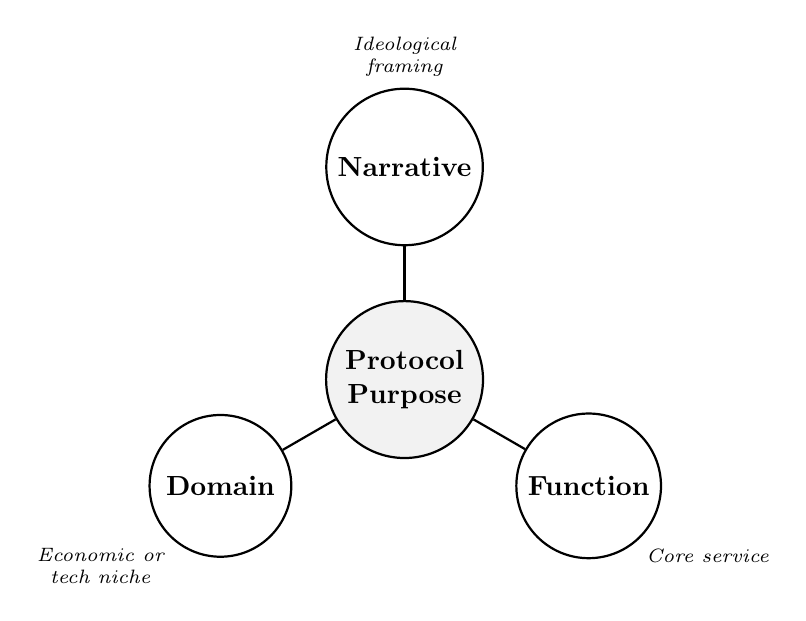
\begin{tikzpicture}[
    main/.style={circle, draw=black, thick, minimum size=1.6cm, align=center, font=\bfseries, fill=gray!10},
    outer/.style={circle, draw=black, thick, minimum size=1.8cm, align=center, font=\bfseries, fill=white},
    desc/.style={font=\scriptsize\itshape, align=center},
    line/.style={thick}
]

% Main center node
\node[main] (center) at (0,0) {Protocol\\Purpose};

% Outer nodes (closer radius)
\node[outer] (narrative) at (90:2.7) {Narrative};
\node[outer] (domain) at (210:2.7) {Domain};
\node[outer] (function) at (330:2.7) {Function};

% Connecting lines
\draw[line] (center) -- (narrative);
\draw[line] (center) -- (domain);
\draw[line] (center) -- (function);

% Descriptions
\node[desc, above=0.02cm of narrative] {Ideological \\ framing};
\node[desc, below left=0.02cm and -0.05cm of domain] {Economic or \\ tech niche};
\node[desc, below right=0.02cm and -0.05cm of function] {Core service};

\end{tikzpicture}
\caption{Three dimensions of protocol purpose: domain, narrative, and function. Effective blockchain networks integrate all three.}
\label{fig:purpose_triangle}
\end{figure}




%------------------------------
\subsection*{2. Incentives}

A blockchain protocol must not only offer a valuable service, but also align the economic behavior of participants with the network’s goals. Incentive mechanisms are the tools through which this alignment is achieved. They provide direct economic rewards that encourage validators, stakers, developers, and users to contribute resources, maintain consensus, and extend the protocol’s utility over time \citep{biais2020blockchain, saleh2021blockchain, singh2025blockchain}.

Incentives may take several forms:

\begin{itemize}
    \item \textit{Protocol-level emissions} (e.g., block rewards, staking yield): native token payouts tied to validation or consensus activities \citep{gans2019economics, catalini2020some}.

    \item \textit{Usage-based fees} (e.g., gas payments, inference compensation): payments triggered by resource consumption or service provision within the network \citep{cong2021tokenomics, huberman2021monetizing}.

    \item \textit{Performance-based allocation mechanisms} (e.g., Bittensor's Yuma Consensus): algorithmic rules that distribute protocol emissions according to measured contribution quality, aggregating stake-weighted peer evaluations to decide which participants are rewarded \citep{rao2020bittensor, yuma2025yuma}. Although named a ``consensus,'' such mechanisms allocate rewards rather than produce blocks or finalize state, and are therefore incentive machinery in this framework (see the Consensus element below).

    \item \textit{Governance and access rights} (e.g., voting power, validator slots): privileges tied to token holdings or performance that influence future protocol evolution \citep{urquhart2022ethereum, buterin2022proof}.
\end{itemize}

\textit{Value contribution}: Incentives contribute to \textbf{desirability}, the demand-side element of economic scarcity (Equation~\ref{eq:economic_scarcity}). By linking participation to tangible rewards, they transform engagement from voluntary altruism into economically rational behavior. Well-designed incentive structures not only support security and sustainability, but also strengthen long-term token utility by ensuring that value flows back to those who contribute meaningfully to the network’s success \citep{biais2020blockchain, cong2021tokenomics, gans2019economics}.

%-----------------------------
\subsection*{3. Consensus}

Consensus mechanisms enable decentralized systems to maintain a shared, tamper-resistant view of the ledger without relying on a central authority. They determine how new transactions are validated, how blocks are appended to the chain, and how the network responds to adversarial behavior. This process ensures both the integrity and the finality of the system’s state\footnote{The consensus mechanism is the primary determinant of ledger correctness, finality, and resistance to manipulation. Broader aspects of network reliability, including uptime, liveness under load, and responsiveness to faults, are economically significant but arise from the consensus protocol’s liveness guarantees, incentive alignment, and supporting infrastructure. These attributes are therefore treated as integral to consensus reliability rather than as a standalone value element, in line with the framework’s modular structure.}
 \citep{saleh2021blockchain, biais2020blockchain}.

Different protocols implement consensus through distinct trust architectures:

\begin{itemize}
    \item \textit{Proof-of-Work (PoW)} (e.g., Bitcoin): relies on energy-intensive computational puzzles to secure the network and make dishonest behavior economically costly \citep{nakamoto2008bitcoin}.
    
    \item \textit{Proof-of-Stake (PoS)} (e.g., Ethereum): assigns block validation rights in proportion to the amount of capital staked, penalizing malicious behavior by slashing collateral \citep{buterin2022proof}.
    
    \item \textit{Delegated Proof-of-Stake ledger consensus with performance-based reward allocation} (e.g., Bittensor): two functionally distinct mechanisms must be distinguished here. Ledger consensus in the sense of this element, i.e., block production, state synchronization, and finality, is provided by the \textit{Subtensor} blockchain, a Polkadot-SDK-based chain secured by its own validator set under standard staking assumptions \citep{rao2020bittensor}. The subnet reward mechanism, \textit{Yuma Consensus}, which aggregates stake-weighted peer evaluations of machine learning contributions, applies clipping to limit bias, and penalizes misaligned scoring, does not produce blocks or finalize state: it is a \emph{reward-allocation} mechanism that distributes emissions among subnet miners and validators \citep{rao2020bittensor, yuma2025yuma}. (Earlier protocol materials marketed this mechanism under the label \textit{Proof-of-Intelligence}; current protocol documentation has retired that label and refers to the mechanism simply as Yuma Consensus, describing it as a subjective-utility consensus over subnet contributions.) In the five-element framework, Subtensor's ledger consensus therefore belongs to the Consensus element, while Yuma Consensus belongs to the Incentives element, where it determines who is paid for what.

\end{itemize}



\textit{Value contribution}: Consensus mechanisms contribute to \textbf{desirability}, the demand-side pillar of economic scarcity (Equation~\ref{eq:economic_scarcity}). By establishing a credible process for transaction validation and state synchronization, they underpin user trust in the correctness and permanence of the ledger. This trust is a prerequisite for the network to be perceived as reliable and secure, making it desirable for use in value transfer, coordination, and application execution, including, but not limited to, the role of the native token as a medium of exchange, unit of account, or governance asset \citep{catalini2020some, urquhart2022ethereum}.

%------------------------------
\subsection*{4. Tokenomics}

Tokenomics refers to the monetary architecture of a protocol’s native token, encompassing the rules for issuance, supply dynamics, distribution, and in-protocol use cases. These structural features shape both user behavior and market expectations, playing a central role in the token’s economic sustainability \citep{cong2021tokenomics, catalini2020some}.

Key design dimensions include:

\begin{itemize}
    \item \textit{Supply policy}: whether the token supply is capped (e.g., Bitcoin, Bittensor), inflationary (e.g., Ethereum post-Merge), or deflationary through burning or base-fee mechanisms \citep{nakamoto2008bitcoin, rao2023bittensor, buterin2022proof}.

    \item \textit{Token utility}: whether tokens are required for executing transactions, staking to secure the network, accessing decentralized services, or participating in governance \citep{buterin2022proof, catalini2020some, urquhart2022ethereum}.

    \item \textit{Distribution logic}: how tokens enter circulation (e.g., block rewards, staking emissions, airdrops, vesting schedules, or contribution-based payouts such as inference scoring) \citep{gans2019economics, cong2021tokenomics, rao2023bittensor}.
\end{itemize}

\textit{Value contribution}: Tokenomics contributes to \textbf{physical scarcity}, the supply-side condition for economic scarcity (Equation~\ref{eq:economic_scarcity}). By defining how tokens are created, used, and retired, monetary design influences expectations of long-term value retention and the credibility of the asset as a store of value. Disciplined and transparent tokenomics strengthen monetary policy credibility, support incentive alignment, and limit speculative distortion \citep{gans2019economics, huberman2021monetizing}.

%------------------------------
\subsection*{5. Network Effects}

The value of a blockchain protocol arises not only from the services it provides but also from how user participation scales the system’s utility. A well-designed network leverages growth to generate nonlinear returns, amplifying desirability as adoption increases. This phenomenon, known as the network effect, is not incidental; it is embedded by design in the protocol’s architecture, interaction model, and token utility \citep{gans2019economics, huberman2021monetizing, catalini2020some}.

Different blockchain ecosystems encode different types of network effects, which can be formalized heuristically as functions of the user base \( u \):

\begin{itemize}
    \item \textit{Sarnoff's Law (linear)}: \( V(u) = \alpha \cdot u \). Value increases proportionally with the number of users; each additional participant contributes a fixed marginal value.

    \item \textit{Metcalfe's Law (quadratic)}: \( V(u) = \beta \cdot u^2 \). Value increases with the number of potential user-to-user connections. Bitcoin and Ethereum generally approximate this structure, as they enable bilateral value exchange through peer-to-peer transaction layers \citep{gans2019economics, huberman2021monetizing}.

    \item \textit{Reed's Law (exponential)}: \( V(u) = \gamma \cdot 2^u \). Value grows with the number of possible subgroups or coalitions among users. Composable ecosystems such as Bittensor, with subnet architectures and collaborative inference markets, are the natural candidates for this regime \citep{rao2023bittensor, gregory2025token}; whether they realize it is an empirical question, and the valuation analysis of Section~5 therefore adopts a common quadratic baseline for all networks and treats superlinear scaling only as a sensitivity scenario.
\end{itemize}


Here, \( u \) denotes the number of users, and \( \alpha, \beta, \gamma \) are scaling constants normalized to 1 in the illustrative figure below. These models are not mutually exclusive; a single protocol may exhibit multiple growth dynamics depending on its dominant interaction logic, whether broadcasting, peer-to-peer exchange, or collective subgroup formation.

\textit{Value contribution}: Network effects simultaneously enhance \textbf{desirability} and \textbf{physical scarcity}. As user participation increases, the network becomes more functional, attractive, and widely adopted, raising its desirability. At the same time, growing demand intensifies competition for constrained resources such as blockspace, bandwidth, or token supply, thereby increasing scarcity. In this sense, network effects operate through the interaction of desirability and scarcity, amplifying their joint contribution within the valuation function \( V_t = F(D_t, S_t) \) as in Equation~\ref{eq:economic_scarcity}, which can be conceptualized multiplicatively as \( V_t \propto D_t \cdot S_t \). Strong network effects therefore magnify economic scarcity on both margins, increasing perceived value while reinforcing structural exclusivity.



Figure~\ref{fig:network_effects} below visualizes the growth behavior under each scaling regime.


\begin{figure}[H]
\centering

% --- Left panel: log y-axis full range ---
\begin{minipage}{0.48\textwidth}
\centering
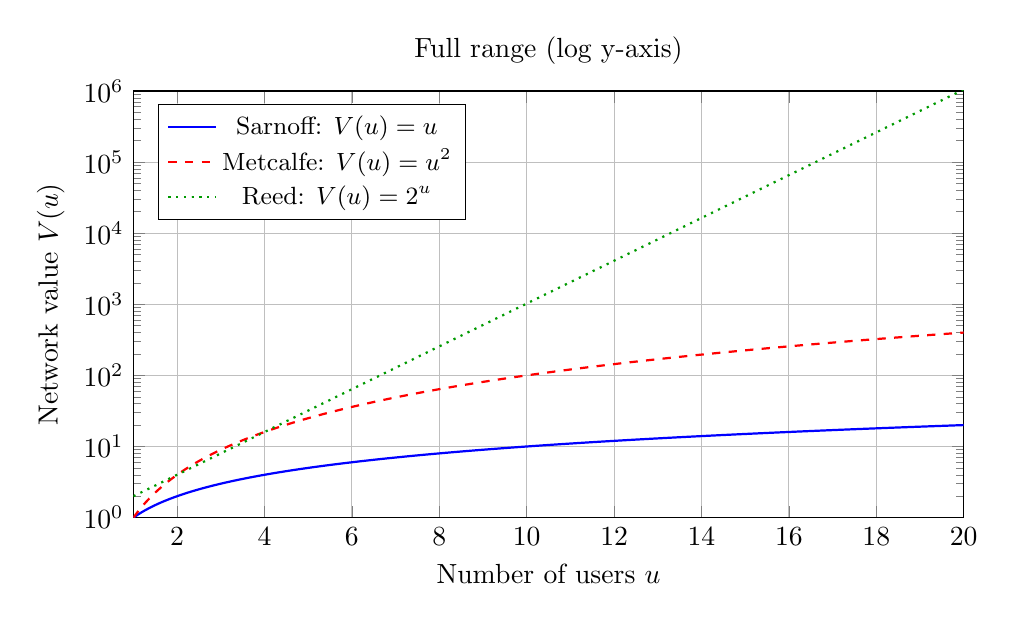
\begin{tikzpicture}
\begin{semilogyaxis}[
    xlabel={Number of users \( u \)},
    ylabel={Network value \( V(u) \)},
    xmin=1, xmax=20,
    ymin=1, ymax=1e6,
    samples=200,
    grid=major,
    legend pos=north west,
    width=\linewidth,
    height=7cm,
    legend style={font=\small},
    yticklabel style={/pgf/number format/fixed},
    title={Full range (log y-axis)}
]
% Sarnoff: Linear
\addplot[blue, thick, domain=1:20] {x};
\addlegendentry{Sarnoff: \( V(u)=u \)}

% Metcalfe: Quadratic
\addplot[red, thick, dashed, domain=1:20] {x^2};
\addlegendentry{Metcalfe: \( V(u)=u^2 \)}

% Reed: Exponential
\addplot[green!60!black, thick, dotted, domain=1:20] {2^x};
\addlegendentry{Reed: \( V(u)=2^u \)}
\end{semilogyaxis}
\end{tikzpicture}
\end{minipage}
\hfill
% --- Right panel: early-stage zoom ---
\begin{minipage}{0.48\textwidth}
\centering
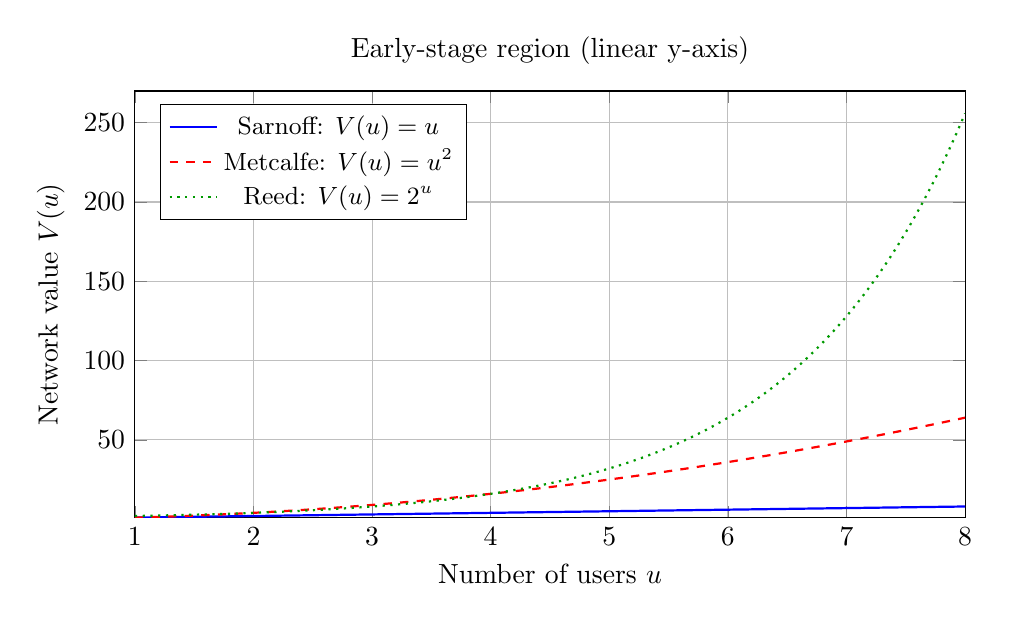
\begin{tikzpicture}
\begin{axis}[
    xlabel={Number of users \( u \)},
    ylabel={Network value \( V(u) \)},
    xmin=1, xmax=8,
    ymin=1, ymax=270,
    samples=200,
    grid=both,
    legend pos=north west,
    width=\linewidth,
    height=7cm,
    legend style={font=\small},
    title={Early-stage region (linear y-axis)}
]
% Sarnoff
\addplot[blue, thick, domain=1:8] {x};
\addlegendentry{Sarnoff: \( V(u)=u \)}

% Metcalfe
\addplot[red, thick, dashed, domain=1:8] {x^2};
\addlegendentry{Metcalfe: \( V(u)=u^2 \)}

% Reed
\addplot[green!60!black, thick, dotted, domain=1:8] {2^x};
\addlegendentry{Reed: \( V(u)=2^u \)}
\end{axis}
\end{tikzpicture}
\end{minipage}

\caption{Network value under Sarnoff, Metcalfe, and Reed scaling. Left: full range on a logarithmic y-axis to capture relative growth. Right: early-stage region (\(u \in [1,8]\)) on a linear y-axis to make small-scale differences visible.}
\label{fig:network_effects}
\end{figure}



%----------------------------------
\subsection{Interdependence of Value Elements}

The five structural elements identified in this framework, \textit{Purpose}, \textit{Incentives}, \textit{Consensus}, \textit{Tokenomics}, and \textit{Network Effects}, do not operate in isolation. Blockchain value is a systemic outcome shaped by how these elements interact to support or constrain one another. A protocol’s ability to create and sustain economic scarcity depends not only on the quality of individual components but also on the coherence of their integration \citep{gans2019economics, canidio2021tokens, catalini2020some}.


For example, a strong \textit{Purpose} requires well-aligned \textit{Incentives} to attract the right participants and sustain engagement. A protocol that enables decentralized knowledge production, such as Bittensor, must reward the generation of useful outputs rather than mere presence or computational effort \citep{rao2023bittensor}. Similarly, \textit{Tokenomics} governs the viability of incentives: if a protocol relies on inflationary rewards to motivate participation but lacks sufficient token utility, its incentive structures may erode over time \citep{cong2021tokenomics, huberman2021monetizing}.

\textit{Consensus} and \textit{Tokenomics} are also intertwined. In Proof-of-Stake systems like Ethereum, network security depends on the economic value and distribution of the staking token \citep{buterin2022proof}. Weaknesses in issuance policy can undermine confidence in long-term value retention, indirectly affecting consensus security. Likewise, incentive design and consensus interact: validators behave honestly only if rewards outweigh the costs of deviation \citep{saleh2021blockchain}.

\textit{Network Effects} emerge when user adoption amplifies desirability, but their strength depends on \textit{Purpose} and usability. Poor design or weak incentives can prevent early users from becoming long-term participants, breaking the compounding feedback loop needed to achieve scale \citep{gans2019economics, urquhart2022ethereum}. Conversely, rapid adoption can create congestion that must be addressed through scalable consensus and sound resource pricing, linking network effects back to consensus and tokenomics.

In practice, these interactions form a tightly coupled system (Figure~\ref{fig:element_interaction}). Misalignment between even two components can impair the overall value proposition, while well-integrated designs reinforce one another to generate sustainable economic scarcity, as formalized in Equation~\ref{eq:economic_scarcity}.

\begin{figure}[H]
\centering
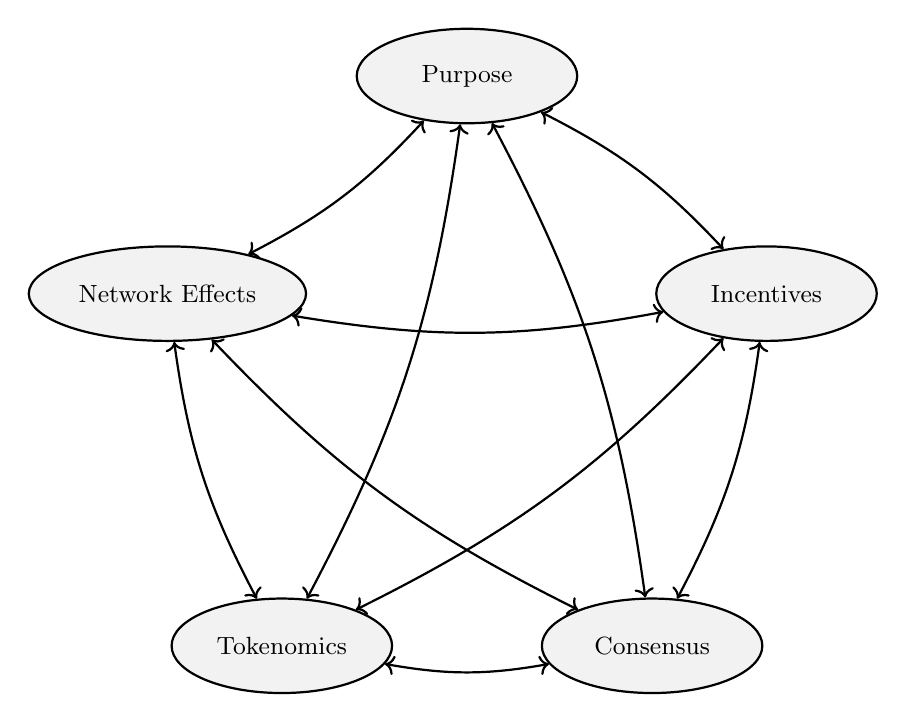
\begin{tikzpicture}[node distance=3cm, every node/.style={font=\small}]
\tikzstyle{element}=[ellipse, draw=black, fill=gray!10, thick, 
  minimum width=2.8cm, minimum height=1.2cm]

\node[element] (P) at (90:4cm) {Purpose};
\node[element] (I) at (18:4cm) {Incentives};
\node[element] (C) at (306:4cm) {Consensus};
\node[element] (T) at (234:4cm) {Tokenomics};
\node[element] (N) at (162:4cm) {Network Effects};

\path[<->, thick] (P) edge[bend left=10] (I);
\path[<->, thick] (P) edge[bend left=10] (C);
\path[<->, thick] (P) edge[bend left=10] (T);
\path[<->, thick] (P) edge[bend left=10] (N);
\path[<->, thick] (I) edge[bend left=10] (C);
\path[<->, thick] (I) edge[bend left=10] (T);
\path[<->, thick] (I) edge[bend left=10] (N);
\path[<->, thick] (C) edge[bend left=10] (T);
\path[<->, thick] (C) edge[bend left=10] (N);
\path[<->, thick] (T) edge[bend left=10] (N);

\end{tikzpicture}
\caption{The five foundational elements of blockchain value form a fully interdependent system. Bidirectional arrows represent mutual influence. Network value emerges from the internal coherence and feedback dynamics among Purpose, Incentives, Consensus, Tokenomics, and Network Effects.}
\label{fig:element_interaction}
\end{figure}

\begin{tcolorbox}[title=\textbf{Remark: Blockchain Value as a Systemic Outcome}]
The five elements form a structurally interdependent system. Value emerges not from their independent strengths but from how they reinforce one another. A protocol with excellent tokenomics but unclear purpose, or strong consensus without incentive alignment, will struggle to sustain economic scarcity. Robust valuation requires cohesion across all architectural components.
\end{tcolorbox}



%----------------------------------
\subsection{Summary}

The five structural elements, \textit{Purpose}, \textit{Incentives}, \textit{Consensus}, \textit{Tokenomics}, and \textit{Network Effects}, jointly determine a blockchain network's capacity to generate economic value. Each contributes either to desirability, physical scarcity, or both, as formalized in Equation~\ref{eq:economic_scarcity}. Table~\ref{tab:value_elements} summarizes these elements, their functional definitions, and how each contributes to the emergence of economic scarcity within blockchain systems.

\begin{table}[h]
\centering
\caption{Blockchain Value Elements and Their Contribution to Economic Scarcity}
\label{tab:value_elements}
\renewcommand{\arraystretch}{1.4}
\begin{tabular}{@{}L{4.2cm}L{5.4cm}L{5.6cm}@{}}
\toprule
\rowcolor{gray!15}
\textbf{Element} & \textbf{Definition} & \textbf{Value Contribution (D = Desirability, S = Physical Scarcity)} \\
\midrule
\textbf{Purpose} & The economically or socially meaningful service the protocol delivers. & Drives \textbf{D} by generating user demand and anchoring token utility. \\

\textbf{Incentives} & Mechanisms that reward participation and contribution (e.g., staking, fees). & Reinforces activity and trust through aligned self-interest; supports \textbf{D}. \\

\textbf{Consensus} & Protocol rules ensuring agreement over system state (e.g., PoW, PoS). & Establishes correctness and resistance to manipulation; supports both \textbf{D} and network integrity. \\

\textbf{Tokenomics} & The monetary and supply policy of the native token. & Shapes expectations of \textbf{S} through controlled issuance and utility design. \\

\textbf{Network Effects} & Structural law relating user growth to value (e.g., Sarnoff, Metcalfe, Reed). & Amplifies \textbf{D} via scalable interactions; increases \textbf{S} through congestion and exclusivity. \\
\bottomrule
\end{tabular}
\end{table}

\begin{tcolorbox}[title=\textbf{Remark: Sufficiency and Modularity of the Five Elements}]
The five structural elements span the fundamental forces driving blockchain valuation through the lens of economic scarcity (Equation~\ref{eq:economic_scarcity}) and align with the principal layers of distributed system design.

Attributes often discussed as separate drivers, such as governance, interoperability, or composability, are analytically subsumed within these elements: governance within Incentives and Consensus, interoperability and composability within Network Effects and Purpose.

This modular scope keeps the framework parsimonious, adaptable, and applicable across both economic analysis and system architecture, forming an explicit \textit{architecture--valuation bridge}.
\end{tcolorbox}

\begin{tcolorbox}[title=\textbf{Remark: Operational Reliability and Downtime}]
Operational attributes such as uptime, liveness under load, responsiveness to faults, and planned upgrade paths derive their economic relevance from how they influence trust (Consensus) and retention (Incentives, Tokenomics).

Rather than being treated as standalone elements, these factors are embedded in the existing framework, reflecting their role as enablers of sustained economic scarcity through dependable protocol performance.
\end{tcolorbox}



To ground the framework in concrete examples, we next examine three blockchain protocols that represent distinct paradigm shifts in both technical architecture and economic value generation. By mapping Bitcoin, Ethereum, and Bittensor onto the five structural elements, we show how differences in design choices translate into differences in the generation and sustainability of economic scarcity.



%-----------------------------------
\subsection{Case Study: Bitcoin, Ethereum, and Bittensor}
\label{subsec:five_element_case_study}

To demonstrate the applicability of the five-element valuation framework, we examine three blockchain protocols, Bitcoin (BTC), Ethereum (ETH), and Bittensor (TAO), that mark clear paradigm shifts in how economic scarcity is generated and sustained. Each reflects a distinct architectural approach across \textit{Purpose}, \textit{Incentives}, \textit{Consensus}, \textit{Tokenomics}, and \textit{Network Effects}:

\begin{itemize}
    \item \textbf{Bitcoin} adopts \textit{Proof-of-Work} (PoW), using energy expenditure to constrain access and secure consensus \citep{nakamoto2008bitcoin, gans2019economics}.
    \item \textbf{Ethereum} transitioned to \textit{Proof-of-Stake} (PoS), securing the network through bonded capital and dynamic monetary policy \citep{buterin2022proof, schar2021defi}.
    \item \textbf{Bittensor} runs delegated Proof-of-Stake ledger consensus on its Subtensor chain, while allocating economic rewards through \textit{Yuma Consensus}, a stake-weighted peer-evaluation mechanism for machine learning contributions (described in earlier protocol materials as \textit{Proof-of-Intelligence}) \citep{rao2023bittensor}.
\end{itemize}

Table~\ref{tab:case_study_elements} summarizes the structural profile of each protocol across the five foundational value dimensions.

\begin{table}[H]
\centering
\caption{Comparative structural profile of Bitcoin (BTC), Ethereum (ETH), and Bittensor (TAO) across the five value elements, as of 5 August 2025. The Tokenomics row anticipates the scarcity components quantified in Table~\ref{tab:scarcity_summary}; the Network Effects row anticipates the adoption measures of Table~\ref{tab:user_adoption}.}
\label{tab:case_study_elements}
\renewcommand{\arraystretch}{1.4}
\begin{tabular}{@{}L{3.5cm}L{4.1cm}L{4.1cm}L{4.1cm}@{}}
\toprule
\rowcolor{gray!15}
Element & Bitcoin (BTC) & Ethereum (ETH) & Bittensor (TAO) \\
\midrule
Purpose & Digital gold; decentralized store of value \citep{nakamoto2008bitcoin, huberman2021monetizing} & Global smart contract platform \citep{buterin2022proof, cong2021tokenomics} & Decentralized machine learning inference and ranking \citep{rao2023bittensor} \\
Incentives & Block subsidy and transaction fees to PoW miners \citep{nakamoto2008bitcoin} & Staking rewards and priority fees to validators \citep{buterin2022proof} & Emissions allocated to subnet miners and validators by Yuma Consensus (stake-weighted peer evaluation) \citep{rao2023bittensor} \\
Consensus & Proof-of-Work \citep{nakamoto2008bitcoin} & Proof-of-Stake with slashing \citep{buterin2022proof} & Subtensor chain: delegated Proof-of-Stake ledger consensus (block production and finality) \citep{rao2020bittensor} \\
Tokenomics & Hard cap of 21M; deterministic halving schedule; no protocol burn \citep{nakamoto2008bitcoin} & No hard cap; stable post-Merge issuance; EIP-1559 base-fee burn \citep{buterin2022proof} & Algorithmic 21M cap; halving-based emission decay; registration fees recycled rather than burned \citep{rao2023bittensor} \\
Network Effects & Monetary network; about 1M daily active addresses \citep{glassnodeBTC} & Composability and DeFi ecosystem; about 0.6M daily active addresses \citep{glassnodeETH} & Subnet modularity; about 33k registered neurons across 128 subnets \citep{taostats_accounts} \\
\bottomrule
\end{tabular}
\end{table}

These three protocols were chosen not only for their market relevance but because each represents a distinct paradigm shift: Bitcoin established fixed-supply, proof-of-work monetary systems; Ethereum introduced programmable, composable smart contracts; and Bittensor pioneered performance-based reward allocation for decentralized AI. In the following section, we map these profiles into the economic scarcity framework to show how differences in design translate into differences in value generation.


%%%%%%%%%%%%%%%%%%%%%%%%%%%%%%%%%%%%%%%%%%%%%%%%%%%%%%%%%
\section{The Native Token}
\label{sec:native_token}

The native token is the operational and economic nucleus of a blockchain network. Unlike traditional securities such as equity or debt, it does not confer ownership rights, contractual claims, or dividend entitlements. Instead, it functions as a protocol-native coordination instrument that enables access, secures consensus, aligns incentives, enforces monetary policy, and scales adoption \citep{cong2021tokenomics, catalini2020some, gans2019economics}. 

In the context of this framework, the native token binds together the five structural value elements from Section~\ref{sec:framework_elements}:

\begin{itemize}
    \item \textbf{Purpose:} mediates access to the protocol’s primary service. Examples include censorship-resistant transfers in Bitcoin \citep{nakamoto2008bitcoin}, programmable computation in Ethereum \citep{buterin2022proof}, and decentralized AI inference in Bittensor \citep{rao2023bittensor}. Holding the token can also signal long-term belief in the protocol’s utility \citep{huberman2021monetizing, urquhart2022ethereum}.
    
    \item \textbf{Incentives:} delivers rewards for economically meaningful participation such as mining, staking, validating, or fulfilling protocol-specific roles \citep{saleh2021blockchain, biais2020blockchain, catalini2020some}.
    
    \item \textbf{Consensus:} represents either a cost of computation (Proof-of-Work), a stake at risk (Proof-of-Stake), or a verifiable performance signal (Bittensor's Yuma Consensus) \citep{nakamoto2008bitcoin, buterin2022proof, rao2023bittensor}.
    
    \item \textbf{Tokenomics:} implements the protocol’s monetary architecture, including issuance rules, inflation schedules, caps, burns, and distribution \citep{cong2021tokenomics, gans2019economics}.
    
    \item \textbf{Network Effects:} acts as the medium through which user growth translates into adoption, utility, and congestion, reinforcing scarcity \citep{huberman2021monetizing, catalini2020some}.
\end{itemize}

\begin{tcolorbox}[title=\textbf{Definition (Functional Role of the Native Token)}]
A blockchain network’s native token performs five core functions:
\begin{enumerate}
    \item Grants access to purpose-driven services.
    \item Aligns participant incentives through rewards.
    \item Secures consensus via stake, effort, or verifiable contribution.
    \item Implements monetary rules that define scarcity.
    \item Mediates adoption and network effects through usage and holding.
\end{enumerate}
\end{tcolorbox}

These functions are mutually reinforcing. The token acts as the economic interface between technical architecture and valuation outcomes, forming an explicit \textit{architecture--valuation bridge} (Figure~\ref{fig:native_token_coordination}).

A detailed comparison between native blockchain tokens and traditional equity instruments, including their respective legal, economic, and architectural foundations, is provided in Appendix~\ref{appendix:tokens_vs_equity}.

\subsection{Value Capture by the Native Token}
\label{subsec:value_capture}

The five elements describe the conditions under which a \emph{network} can generate economic scarcity; whether that scarcity accrues to the \emph{native token} is a further design question. Network usefulness translates into token value only through specific capture channels: (i) \textit{holding requirements}, where accessing the service or securing the network requires acquiring and locking the token (staking, bonding, validator collateral); (ii) \textit{fee flows and burns}, where usage generates fees paid in, or permanently removing, the token (e.g., Ethereum's EIP-1559 base-fee burn); (iii) \textit{circulation velocity}, since a token that is immediately resold after use supports less value per unit of activity than one that is held, a point formalized in monetary treatments of token velocity \citep{cong2021tokenomics}; and (iv) \textit{issuance-funded incentives}, which dilute holders when service provision is paid from new emissions rather than user fees. A network can be useful and yet capture little value in its token if velocity is high and no holding requirement binds; conversely, aggressive capture mechanisms can tax usage and suppress adoption.

Our framework treats these channels as design properties summarized within the Tokenomics element rather than modeling them explicitly: the valuation form of Section~\ref{sec:valuation_framework} takes the mapping from network activity to token demand as given. Making value capture endogenous, for instance by modeling velocity and fee flows jointly with adoption as in \citet{cong2021tokenomics}, is a natural extension and a limitation of the present, structural approach.


\begin{figure}[H]
\centering
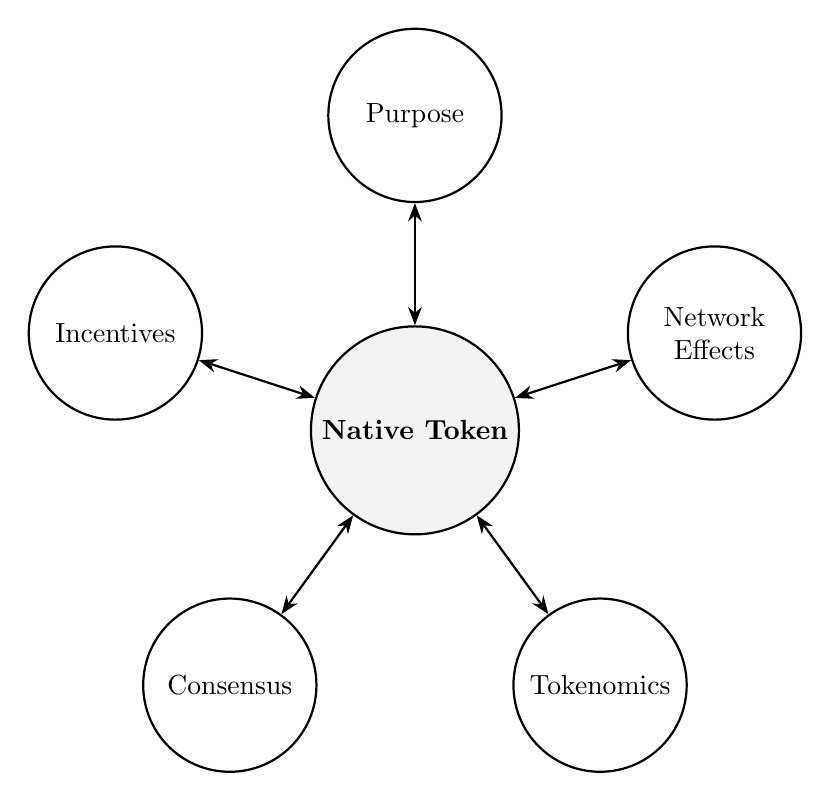
\begin{tikzpicture}[
    element/.style={circle, draw=black, thick, minimum size=2.2cm, align=center},
    center/.style={circle, draw=black, thick, fill=gray!10, minimum size=2.6cm, align=center, font=\bfseries},
    arrow/.style={thick, <->, >=Stealth}
]
% Outer nodes
\node[element] (purpose) at (90:4) {Purpose};
\node[element] (incentives) at (162:4) {Incentives};
\node[element] (consensus) at (234:4) {Consensus};
\node[element] (tokenomics) at (306:4) {Tokenomics};
\node[element] (network) at (18:4) {Network\\Effects};

% Center node
\node[center] (token) at (0,0) {Native Token};

% Arrows
\draw[arrow] (purpose) -- (token);
\draw[arrow] (incentives) -- (token);
\draw[arrow] (consensus) -- (token);
\draw[arrow] (tokenomics) -- (token);
\draw[arrow] (network) -- (token);
\end{tikzpicture}
\caption{The native token integrates the five core value elements. Design choices in Purpose, Incentives, Consensus, Tokenomics, and Network Effects both shape and depend on token functionality.}
\label{fig:native_token_coordination}
\end{figure}

\begin{tcolorbox}[title=\textbf{Remark: Investment Appeal as Emergent Integration}]
Investment demand for a native token reflects confidence in the coherence of its overall architecture. While rooted in purpose, sustainable value arises from credible alignment across all five structural elements. This integration ensures that the token is not only functional within the protocol but also viable as a long-term store of value.
\end{tcolorbox}





%%%%%%%%%%%%%%%%%%%%%%%%%%%%%
\section{Blockchain Network Valuation}
\label{sec:valuation_framework}

As introduced in Equation~\ref{eq:structural_valuation}, we approximate network value as the product of three components: desirability \( D_t \), physical scarcity \( S_t \), and scaled user adoption via network effects. For clarity, we restate the equation below:

\begin{equation*}
V_t \approx D_t \cdot S_t \cdot u_t^{\alpha}
\end{equation*}

This formulation captures the idea that a blockchain protocol becomes economically valuable when a credible and useful function is made scarce and distributed at scale. In what follows, we model physical scarcity \( S_t \) and user adoption \( u_t \) using protocol-level data, and then infer desirability \( D_t \) as the residual driver of market value. For empirical work, \( u_t \) enters in normalized form, \( \tilde{u}_t = u_t / u_0 \); Section~5.3 states this convention and its implications for cross-protocol comparison.

\begin{tcolorbox}[title=\textbf{Remark: Valuation Framework versus Valuation Attribution}]
A distinction governs the empirical work of this section. Equation~\eqref{eq:structural_valuation} is a \emph{valuation framework}: it states what determines value. The exercises below do not produce an independent appraisal that could be compared against the market price; they \emph{decompose the observed market value} into the share explained by measured scarcity and adoption and the residual share attributed to implied desirability. The scarcity index of Section~5.1 is accordingly a structural score, not a price, and the implied desirability of Section~5.3 is calibrated to market capitalization by construction, in the way implied volatility is calibrated to option prices. A standalone valuation would require an exogenous estimate of desirability, which this paper does not claim to provide.
\end{tcolorbox}

%------------------------------------------------------
\subsection{Valuing Physical Scarcity}

Physical scarcity plays a central role in blockchain valuation by capturing the protocol’s structural commitment to monetary constraint. Unlike traditional financial systems where supply policies are subject to discretionary control, blockchain networks encode monetary discipline directly into their architecture. This section develops a quantitative framework for assessing and comparing physical scarcity across protocols, linking design features and inflation dynamics to a unified scarcity score.

\subsubsection{Theoretical Framework}

Physical scarcity refers to the degree to which a blockchain network is structurally protected against uncontrolled token expansion. This concept captures the extent to which monetary supply is disciplined by the protocol, both through its encoded rules and its resistance to discretionary change.

We quantify physical scarcity \( S_t \) as a function of two components: the network's inflation rate \( \pi_t \), and a structural discipline coefficient \( \kappa \), which summarizes the robustness of supply governance:

\begin{equation}
S_t = \kappa \cdot (1 - \pi_t)^{\beta},
\label{eq:physical_scarcity}
\end{equation}

\noindent where:
\begin{itemize}
    \item \( S_t \) is the physical scarcity score at time \( t \),
    \item \( \pi_t \) is the annualized token inflation rate, expressed as a decimal,
    \item \( \beta \) is a sensitivity parameter controlling how strongly inflation reduces perceived scarcity,
    \item \( \kappa \) reflects the protocol’s structural commitment to supply constraint.
\end{itemize}

\subsubsection{Structural Discipline Assessment}

To evaluate \( \kappa \), we assess five core elements of protocol design that determine monetary rigidity:

\begin{itemize}
    \item \textbf{Cap Enforcement (\( C \))}: Whether a maximum token supply exists and is credibly enforced.
    \item \textbf{Emission Rigidity (\( E \))}: The determinism and predictability of the issuance schedule.
    \item \textbf{Burn Mechanism (\( B \))}: Whether tokens are permanently removed from circulation through endogenous processes.
    \item \textbf{Governance Mutability (\( G \))}: The ease with which monetary rules can be changed.
    \item \textbf{Normative Resistance (\( R \))}: The social or technical cost of violating monetary constraints.
\end{itemize}

These scores are normalized on a 0–1 scale. The structural coefficient \( \kappa \) is then computed as the unweighted average of the five components:

\begin{equation}
\kappa = \frac{1}{5}(C + E + B + G + R).
\label{eq:kappa}
\end{equation}

\subsubsection{Empirical Scoring Methodology}

To operationalize our framework, we decompose physical scarcity into two logical tiers:  
\begin{itemize}
    \item \textbf{Structural design components}: These include Cap Enforcement (\(C\)), Emission Rigidity (\(E\)), and Burn Mechanism (\(B\)). They represent the protocol’s encoded monetary rules, i.e., what exists in the code and issuance schedule.
    \item \textbf{Reliability modifiers}: Governance Mutability (\(G\)) and Normative Resistance (\(R\)) capture how easily structural rules can be altered, either through formal governance processes or informal social/political pressure.
\end{itemize}

We assign values to each of the five components on a 0--1 scale according to the scoring rubric in Table~\ref{tab:scoring_rubric}, drawing on protocol documentation, governance design, and observed historical behavior; intermediate values interpolate between the stated anchors. Two conventions deserve emphasis. \textit{Burn Mechanism} scores strictly the \emph{permanent removal of circulating tokens} by a protocol mechanism; reduced future issuance (halvings, emission decay) is not a burn and is credited under \textit{Emission Rigidity}. \textit{Governance Mutability} is scored so that higher values indicate greater \emph{difficulty} of changing monetary rules. The per-protocol scores (Table~\ref{tab:scarcity_summary}) and their written rationale are recorded in the reproduction repository. The scores remain expert assessments on a documented rubric rather than measurements, and we treat this as a limitation; its consequences are bounded in Appendix~\ref{appendix:alpha_sensitivity}, which shows that the cross-protocol orderings of \( S_t \) and of implied desirability are unchanged when any single component score is shifted by \( \pm 0.15 \), and are preserved in 97\% and 100\% of draws, respectively, when all fifteen scores are perturbed jointly.

\begin{table}[H]
\centering
\caption{\textbf{Scoring Rubric for the Structural Scarcity Components.} Anchor definitions for scores of 0, 0.5 and 1; intermediate values interpolate.}
\label{tab:scoring_rubric}
\renewcommand{\arraystretch}{1.3}
\small
\begin{tabular}{@{}>{\raggedright\arraybackslash}p{2.6cm} >{\raggedright\arraybackslash}p{3.9cm} >{\raggedright\arraybackslash}p{4.2cm} >{\raggedright\arraybackslash}p{4.2cm}@{}}
\toprule
\rowcolor{gray!15}
\textbf{Component} & \textbf{Score 0} & \textbf{Score 0.5} & \textbf{Score 1} \\
\midrule
Cap Enforcement (\(C\)) & No maximum supply & Cap exists but is modifiable through ordinary governance, or is not yet socially entrenched & Hard-coded cap, credibly enforced and socially entrenched \\
Emission Rigidity (\(E\)) & Discretionary issuance & Rule-based issuance that is readily amendable & Fully deterministic schedule (including programmed halvings or decay) \\
Burn Mechanism (\(B\)) & No protocol mechanism permanently removes circulating tokens & Partial or conditional removal; fee mechanisms that mostly recycle rather than destroy tokens & Continuous, usage-linked permanent removal of tokens \\
Governance Mutability (\(G\)) & Monetary parameters changeable by a small group or a single body & Formal multi-body governance with checks (e.g., council and senate) & No formal process; change requires near-universal social consensus \\
Normative Resistance (\(R\)) & No established community norm around monetary rules & Norms forming or contested & Violation of monetary rules widely regarded as illegitimate \\
\bottomrule
\end{tabular}
\end{table}

Inflation data are sourced from publicly available metrics such as \textit{StakingRewards.com} (August 2025) \citep{stakingrewards2025eth}. We set \( \beta = 1.5 \) to moderately penalize inflation while preserving comparability across networks, and apply this value consistently to all three protocols; results under \( \beta \in \{1.0, 2.0\} \) are reported in the reproduction repository and leave the cross-protocol ordering of \( S_t \) unchanged. Equal component weights in Equation~\ref{eq:kappa} are a stated baseline; a weight-sensitivity analysis doubling each component's weight in turn (reported in the repository) preserves the ordering \( \kappa_{\text{BTC}} > \kappa_{\text{ETH}} > \kappa_{\text{TAO}} \) in every case but one: doubling the weight of the burn component places Ethereum, the only protocol in the sample with a genuine burn mechanism, marginally above Bitcoin (\( \kappa \) of 0.700 against 0.667). All observations in this section refer to a 5 August 2025 snapshot; for Bittensor, this falls under the dynamic-TAO (dTAO) subnet-token regime introduced in February 2025 and predates the December 2025 halving and subsequent emission-model changes.

\subsubsection{Case Study: Bitcoin, Ethereum, and Bittensor}

To illustrate the empirical application of our physical scarcity framework, we evaluate three paradigm-defining blockchain protocols: Bitcoin (decentralized money), Ethereum (programmable smart contracts), and Bittensor (decentralized AI infrastructure), each embodying a unique approach to cryptoeconomic design. For each network, we score the five structural components (\( C, E, B, G, R \)) and compute the overall discipline coefficient \( \kappa \) using Equation~\ref{eq:kappa}. Combined with the observed inflation rate \( \pi_t \), we derive the final physical scarcity score \( S_t \) via Equation~\ref{eq:physical_scarcity}.

These results are summarized in Table~\ref{tab:scarcity_summary}, 
which reports the inflation rate, component-level scores, structural coefficient 
\( \kappa \), and derived physical scarcity \( S_t \) for each network.


\begin{table}[H]
\centering
\caption{\textbf{Component-Level Physical Scarcity Scores of Bitcoin (BTC), Ethereum (ETH), and Bittensor (TAO), as of 5 August 2025.} Scores follow the rubric of Table~\ref{tab:scoring_rubric}; \( \beta = 1.5 \).}
\label{tab:scarcity_summary}
\renewcommand{\arraystretch}{1.2}
\small
\begin{tabular}{@{}L{2.2cm} | L{1.5cm}
                |>{\centering\arraybackslash}p{0.6cm}
                >{\centering\arraybackslash}p{0.6cm}
                >{\centering\arraybackslash}p{0.6cm}
                |>{\centering\arraybackslash}p{0.6cm}
                >{\centering\arraybackslash}p{0.6cm}
                |>{\centering\arraybackslash}p{0.8cm}
                >{\centering\arraybackslash}p{0.9cm}@{}}
\toprule
& \textbf{Inflation} & \multicolumn{3}{c|}{\textbf{Structural Design}} 
  & \multicolumn{2}{c|}{\textbf{Reliability}} 
  & \multicolumn{2}{c@{}}{\textbf{Aggregate}} \\
\cmidrule(lr){2-2} \cmidrule(lr){3-5} \cmidrule(lr){6-7} \cmidrule(l){8-9}
\rowcolor{gray!15}
\textbf{Network} & \( \pi_t \) & 
\( C \) & \( E \) & \( B \) & 
\( G \) & \( R \) & 
\( \kappa \) & \( S_t \) \\
\midrule
\textbf{Bitcoin (BTC)}   & 0.017   & 1.00 & 1.00 & 0.00 & 1.00 & 1.00 & 0.80 & 0.780 \\
\textbf{Ethereum (ETH)}  & 0.0069  & 0.60 & 0.80 & 0.80 & 0.50 & 0.70 & 0.68 & 0.673 \\
\textbf{Bittensor (TAO)} & 0.2035  & 0.85 & 0.75 & 0.30 & 0.60 & 0.50 & 0.60 & 0.427 \\
\bottomrule
\end{tabular}
\end{table}



%----------------------------------------
Figure~\ref{fig:kappa_vs_s} compares the overall structural coefficient
\( \kappa \) with the derived physical scarcity score \( S_t \) for the
three networks, highlighting the gap between design rigidity and effective scarcity
once inflation is accounted for.

\begin{figure}[H]
\centering
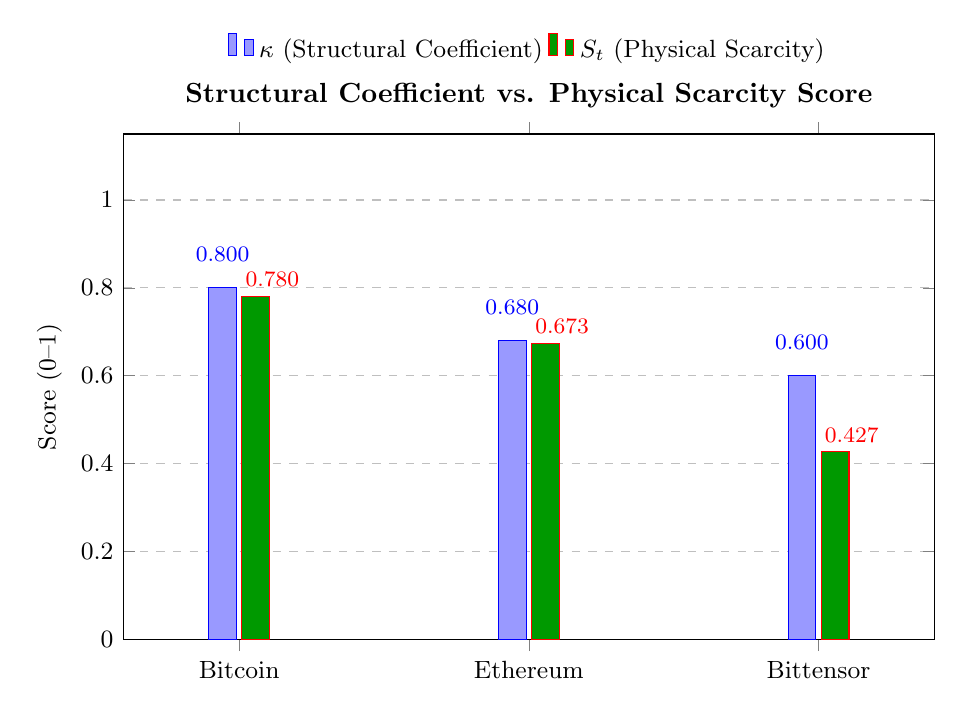
\begin{tikzpicture}
\begin{axis}[
    ybar,
    bar width=10pt,
    width=0.98\textwidth,
    height=8cm,
    enlarge x limits=0.20,
    ylabel={Score (0--1)},
    symbolic x coords={Bitcoin, Ethereum, Bittensor},
    xtick=data,
    xticklabel style={rotate=0, anchor=north, font=\small},
    ymin=0, ymax=1.15,
    title={\textbf{Structural Coefficient vs. Physical Scarcity Score}},
    nodes near coords={\pgfmathprintnumber[fixed, fixed zerofill, precision=3]{\pgfplotspointmeta}},
    legend style={
        at={(0.5,1.12)}, 
        anchor=south, 
        legend columns=2, 
        font=\small,
        draw=none, fill=none
    },
    ymajorgrids=true,
    grid style=dashed,
    tick label style={font=\small},
    ylabel style={font=\small},
]

% Structural Coefficient (\kappa)
\addplot+[
    style={fill=blue!40},
    nodes near coords={\pgfmathprintnumber[fixed, fixed zerofill, precision=3]{\pgfplotspointmeta}},
    every node near coord/.append style={
        font=\footnotesize,
        yshift=6pt,
        color=blue
    }
] coordinates {
    (Bitcoin, 0.80)
    (Ethereum, 0.68)
    (Bittensor, 0.60)
};

% Physical Scarcity (S_t), nudged right
\addplot+[
    style={fill=green!60!black},
    nodes near coords={\pgfmathprintnumber[fixed, fixed zerofill, precision=3]{\pgfplotspointmeta}},
    every node near coord/.append style={
        font=\footnotesize,
        color=red,
        xshift=6pt
    }
] coordinates {
    (Bitcoin, 0.780)
    (Ethereum, 0.673)
    (Bittensor, 0.427)
};

\legend{\( \kappa \) (Structural Coefficient), \( S_t \) (Physical Scarcity)}
\end{axis}
\end{tikzpicture}
\caption{Comparison of structural monetary discipline (\( \kappa \)) and derived physical scarcity score (\( S_t \)) for Bitcoin, Ethereum, and Bittensor.}
\label{fig:kappa_vs_s}
\end{figure}


\paragraph{Bitcoin (BTC).}
Bitcoin receives maximal scores on four of the five dimensions. Its supply cap is hard-coded and immutable (\(C = 1.0\)), the issuance schedule, including its halving cycles, is fully deterministic (\(E = 1.0\)), and governance is intentionally minimalistic and resistant to change (\(G = 1.0\)) \citep{nakamoto2008bitcoin}. Under the strict definition adopted here, however, Bitcoin has no burn mechanism: no protocol process permanently removes circulating BTC (\(B = 0\)); halvings reduce \emph{future issuance} and are credited under Emission Rigidity, and coins lost to inaccessible keys are an accident of custody, not a protocol mechanism \citep{saleh2021blockchain}. Normative resistance to any change in monetary parameters remains maximal (\(R = 1.0\)) \citep{cong2021tokenomics}. These yield \( \kappa = 0.80 \) and \( S_t = 0.780 \). As of August 2025, Bitcoin's annual inflation rate is approximately 1.7\%.

\paragraph{Ethereum (ETH).}
Ethereum scores moderately on most dimensions. It lacks a strict supply cap (\(C = 0.6\)) \citep{ethereumSupplyFAQ}, though its post-Merge issuance curve is relatively stable (\(E = 0.8\)) \citep{buterin2022proof}. Governance is highly flexible (\(G = 0.5\)) \citep{buterin2014ethereum}, enabling rapid protocol upgrades and parameter changes. Ethereum is the one network in our sample with a genuine burn under the strict definition: the EIP-1559 base-fee mechanism permanently removes ETH from circulation (\(B = 0.8\)) \citep{eip1559stats}, and moderate social resistance (\(R = 0.7\)) supports overall monetary credibility. These combine to yield \( \kappa = 0.68 \) and \( S_t = 0.673 \). As of August 2025, Ethereum's annual inflation rate is approximately 0.69\%.

\paragraph{Bittensor (TAO).}
Bittensor defines a hard cap of 21 million TAO tokens, algorithmically enforced (\(C = 0.85\)), with a deterministic halving-based issuance schedule (\(E = 0.75\)) \citep{rao2020bittensor, opentensor2023taoeconomy}. Under the strict burn definition, Bittensor scores low (\(B = 0.30\)): subnet and neuron registration fees are predominantly \emph{recycled} into the future emission pool rather than permanently removed from supply, as reflected in the network's on-chain ``recycled'' accounting \citep{taostats_accounts}, with only limited genuinely burned amounts. Emission decay is a property of the issuance schedule and is credited under \(E\), not \(B\). Governance changes must pass through a hybrid Triumvirate and Senate structure (\(G = 0.6\)) \citep{opentensor_governance}, and as a younger network, Bittensor's normative resistance to monetary changes is still forming (\(R = 0.5\)). Overall, these yield \( \kappa = 0.60 \) and \( S_t \approx 0.427 \). As of August 2025, Bittensor's annual inflation rate is approximately 20.35\% (pre-dating the December 2025 halving).


\vspace{0.3cm}
\paragraph{Interpretation.}

The results highlight significant differences in physical scarcity across networks. \textbf{Bitcoin} remains the benchmark of structural monetary discipline, with encoded constraints and entrenched social norms; its \( \kappa \) of 0.80 rather than a near-perfect score reflects only the strict accounting of the burn component, not any weakness in supply discipline, and illustrates that the five components measure different things rather than a single halo. \textbf{Ethereum}, while more adaptable, sustains moderate scarcity through a genuine burn mechanism (EIP-1559). \textbf{Bittensor} demonstrates commitment to monetary constraint at the protocol level through its cap and emission schedule, but is penalized by its high current inflation, recycling-based (rather than burn-based) fee design, and still-forming governance norms. These findings support the view that physical scarcity is not binary, but a spectrum influenced by both code and community.

%--------------------------------------
\subsection{Valuing User Adoption}

User adoption is a primary driver of blockchain network value. As more participants engage with the protocol, network effects amplify its utility and perceived worth. In Equation~\ref{eq:economic_scarcity}, the interaction term \(F(D_t,S_t)\) captures how desirability and scarcity reinforce one another. In blockchain networks, we operationalize \(F\) through the term \(u_t^\alpha\), where \(u_t\) denotes a proxy for adoption at time \(t\) and \(\alpha\) measures the strength of network effects. This subsection formalizes the role of adoption in our structural valuation framework and introduces empirical methods to measure its impact across different blockchain architectures.


\subsubsection{Theoretical Framework}

In our structural valuation framework, the size and activity of the user base amplify network value through the term \( u_t^\alpha \), where \( u_t \) denotes a proxy for adoption at time \( t \). We restate the core valuation equation:

\[
V_t \approx D_t \cdot S_t \cdot u_t^{\alpha}
\]

The exponent \( \alpha \) governs the strength and character of network effects:

\begin{itemize}
  \item \( \alpha = 1 \): Linear scaling, consistent with \textit{Sarnoff’s Law}, where each user independently contributes value.
  \item \( \alpha = 2 \): Quadratic scaling, per \textit{Metcalfe’s Law}, where value arises from pairwise user interactions.
  \item \( \alpha > 2 \): Superlinear scaling, aligned with \textit{Reed’s Law}, where group formation and composability create disproportionate gains.
\end{itemize}

For cross-protocol comparison we adopt a \emph{common baseline} of \( \alpha = 2 \) for all networks studied. As Section~\ref{sec:valuation_framework} makes precise, implied quantities recovered from Equation~\eqref{eq:structural_valuation} are comparable across protocols only under a shared \((\alpha, u_0)\) convention; protocol-specific exponents would make the cross-protocol ordering an artifact of measurement units. Alternative exponents, including a superlinear scenario for Bittensor and an \( n \log n \) specification in the spirit of \citet{briscoe2006metcalfe}, are treated as sensitivity analyses in Appendix~\ref{appendix:alpha_sensitivity}.

To operationalize \( u_t \) empirically, two complementary proxies are commonly employed:

\begin{itemize}
    \item \textbf{Daily active addresses}: the number of unique wallets that broadcast transactions on a given day. This metric captures short-term engagement and network liveness.
    \item \textbf{Total unique addresses}: the cumulative number of distinct addresses ever observed. This reflects long-term network reach and user acquisition.
\end{itemize}

Both measures can be extracted from public blockchain explorers and analytics platforms, enabling calibration of adoption dynamics and inference of the effective scaling regime (\( \alpha \)) across protocols.

\subsubsection{Case Study: Bitcoin, Ethereum, and Bittensor}

We apply our adoption-based valuation framework to three paradigm-shifting blockchain protocols: Bitcoin (decentralized digital money), Ethereum (programmable smart contracts), and Bittensor (decentralized AI infrastructure). Each represents a distinct architectural and functional evolution in blockchain technology, enabling us to examine how network effects manifest across different user engagement models.

\vspace{0.5em}
\paragraph{Bitcoin (BTC).} 
Bitcoin’s value proposition as decentralized digital money is reflected in its broad and persistent user engagement. As of August 2025, data from \textit{Glassnode} and \textit{Coin Metrics} report between 800{,}000 and 1{,}000{,}000 active addresses per day, while cumulative unique addresses exceed 1.2 billion \citep{glassnodeBTC,bitinfochartsBTC}. Given Bitcoin’s peer-to-peer nature and relatively simple user interactions, the scaling effect is well-approximated by Metcalfe’s Law, suggesting \( \alpha \approx 2 \) \citep{bakhtiar2023network}. This baseline is consistent with empirical studies across multiple cryptocurrencies and provides a stable reference point for cross-protocol comparison.


\paragraph{Ethereum (ETH).}
Ethereum supports smart contracts, DeFi applications, and token issuance, resulting in complex and multi-layered user interactions. Daily active addresses range from 300{,}000 to 600{,}000, while cumulative addresses total around 250 million as of 2025 \citep{glassnodeETH,etherscan}. Like Bitcoin, Ethereum’s value scales with network connectivity, making \( \alpha \approx 2 \) a reasonable baseline for valuation purposes \citep{lee2020measurements}. However, due to its richer composability, empirical data show that short bursts of superlinear growth (\( \alpha > 2 \)) can occur during periods of intense on-chain interaction; we treat these as episodic rather than structural.

\paragraph{Bittensor (TAO).}
Bittensor’s economically active population consists of the miners and validators participating in its incentive mechanism, together with staking wallet holders. Rather than transferring an activity ratio from a structurally different network, we estimate adoption from Bittensor-native quantities observable on \textit{Taostats} as of 5 August 2025 \citep{taostats_accounts}. Our \emph{baseline} is \( u \approx 33{,}000 \): the registered neurons (miner and validator UIDs) across the network's 128 subnets, each capped at 256 UID slots, i.e., the population actually participating in the protocol's incentive mechanism. Because operators may run multiple UIDs or hotkeys, we also carry a conservative \emph{lower bound} of \( u \approx 15{,}000 \) consolidated economic operators, and, since staking wallet holders also constitute economic participants, an \emph{upper bound} of \( u \approx 90{,}000 \) active wallets with balances (roughly 32{,}000 new wallets with balances were added in Q2 2025 alone). The network's cumulative \( \sim \)350{,}000 addresses are reported for context only and are not used as an adoption measure. All desirability results in Section~5.3 are reported across this \([15\text{k}, 90\text{k}]\) range. For the network-effect exponent we use the common baseline \( \alpha = 2 \); Bittensor's recursive, composable subnet architecture plausibly supports stronger-than-pairwise interaction, but we treat superlinear scaling (\( \alpha = 2.5 \)) strictly as a sensitivity scenario, since \citet{briscoe2006metcalfe} in fact argue \emph{against} super-quadratic network value, proposing \( n \log n \) scaling, which we also report as a robustness specification in Appendix~\ref{appendix:alpha_sensitivity}.


\vspace{0.5em}
\paragraph{Interpretive Note.}
Both active and total address counts tend to overstate true user participation, as individuals or entities may control multiple wallets. Without adjustment, this inflates \( u_t \) and thus \( u_t^{\alpha} \), potentially overstating the amplification term \( F(D_t,S_t) \) in Equation~\ref{eq:economic_scarcity}. In turn, this can bias the inferred desirability \( D_t \) downward when back-solving from observed market value. Heuristic clustering methods, such as common-input ownership in Bitcoin or contract-interaction patterns in Ethereum, can partially correct for this overcounting. See \citet{he2022address} and \citet{caringella2024bach} for formal models and tools such as BACH; Ethereum-specific heuristics are discussed in \citet{victor2018ethereum}. Applying such adjustments improves the mapping from observed addresses to economically distinct users, refining both adoption estimates and the desirability inference.


\vspace{0.5em}
\paragraph{Empirical Anchoring.}
The metrics in Table~\ref{tab:user_adoption} provide practical proxies for \( u_t \). Bitcoin and Ethereum both exhibit broad adoption and sustained activity; despite Ethereum's richer composability, empirical studies suggest that superlinear effects are only intermittent, supporting the common quadratic baseline. Bittensor operates on a smaller scale with structurally different dynamics: each participant contributes compute and intelligence rather than merely transactional activity, and its adoption is measured from protocol-native participation counts (registered neurons, consolidated operators, and active wallets) rather than from a ratio transferred from another network. Addresses, economically distinct users, miners, validators, and service consumers are not interchangeable categories; the reported range brackets, rather than resolves, this definitional ambiguity.


\begin{table}[H]
\centering
\caption{\textbf{User Adoption Metrics and Network Scaling Regimes of Bitcoin (BTC), Ethereum (ETH), and Bittensor (TAO), as of 5 August 2025.}}
\label{tab:user_adoption}
\renewcommand{\arraystretch}{1.4}
\begin{tabular}{@{}>{\raggedright\arraybackslash}p{3.5cm} >{\raggedright\arraybackslash}p{4.5cm} >{\raggedright\arraybackslash}p{4.5cm} >{\raggedright\arraybackslash}p{3.5cm}@{}}
\toprule
\rowcolor{gray!15}
\textbf{Network} & \shortstack{\textbf{Total Unique} \\ \textbf{Addresses}} & \shortstack{\textbf{Estimated Active} \\ \textbf{Addresses}} & \shortstack{\textbf{Estimated Network} \\ \textbf{Scaling (\( \alpha \))}} \\
\midrule
\textbf{Bitcoin (BTC)} & \textasciitilde1.2 billion \citep{bitinfochartsBTC} & 1M \citep{glassnodeBTC} & \( \alpha = 2 \) (baseline) \\
\textbf{Ethereum (ETH)} & \textasciitilde250 million \citep{etherscan} & 600K \citep{glassnodeETH} & \( \alpha = 2 \) (baseline) \\
\textbf{Bittensor (TAO)} & \textasciitilde350K \citep{taostats_accounts} & 33K (range 15K--90K)\textsuperscript{a} & \( \alpha = 2 \) (baseline)\textsuperscript{b} \\
\bottomrule
\end{tabular}

\vspace{0.4em}
\footnotesize
\textsuperscript{a}\,Bittensor-native estimates (Taostats, 5 August 2025): baseline = registered neurons across 128 subnets \(\times\) 256 UID slots; lower bound = consolidated multi-UID operators; upper bound = active wallets with balances. \quad
\textsuperscript{b}\,Superlinear (\( \alpha = 2.5 \)) and \( n \log n \) specifications reported as sensitivities in Appendix~\ref{appendix:alpha_sensitivity}.
\end{table}





%--------------------------------------
\subsection{Valuing Desirability}

Desirability \( D_t \) is the first pillar of our valuation framework. It captures the market’s belief in a protocol’s usefulness, credibility, and long-term relevance. Unlike physical scarcity \( S_t \) or user adoption \( u_t \), which can be directly measured, \( D_t \) is latent. It reflects why participants choose to engage with the network, how well incentives sustain that engagement, and whether the system is trusted to deliver its intended function.

\subsubsection{Theoretical Framework}

We model \( D_t \) as a function of three protocol-level dimensions:

\begin{equation}
D_t = f_D(P_t, I_t, C_t),
\label{eq:desirability_1}
\end{equation}

\noindent where:
\begin{itemize}
    \item \( P_t \): the economic or social \textbf{purpose} of the network: the problem it addresses and its relevance within the broader ecosystem,
    \item \( I_t \): the \textbf{incentive structure}, including rewards, costs of participation, and long-term alignment for users and validators,
    \item \( C_t \): the \textbf{credibility of consensus}, meaning the system’s ability to maintain a secure, tamper-resistant, and agreed-upon state.
\end{itemize}

Each dimension shapes desirability by influencing how participants assess the network’s utility and reliability. A protocol with a compelling purpose but weak consensus may be perceived as risky. Conversely, a technically robust protocol without a distinctive purpose may fail to attract sustained participation.

While Equation~\eqref{eq:desirability_1} describes the structural determinants of desirability conceptually, \( D_t \) itself is not directly observable, and we make no claim to \emph{estimate} the function \( f_D \). Instead, we recover an \textbf{implied desirability}: the component of market valuation not explained by measured scarcity and adoption under a stated measurement convention. The construction parallels implied volatility in options pricing, where an unobservable parameter is inferred from market prices given observed inputs and a pricing convention, and is an \emph{attribution} method, not a predictive model. Because it is a residual, implied desirability absorbs, alongside current protocol utility, everything else the structural terms omit: expectations of future utility and adoption, liquidity conditions, speculative demand, and measurement error in \( S_t \) and \( u_t \). This composition is central to its interpretation, particularly for young networks, where expectations can dominate measured fundamentals.

\paragraph{Normalization.}
User counts enter the inversion as the dimensionless ratio \( \tilde{u}_t = u_t / u_0 \), with a single common reference scale \( u_0 = 10^6 \) users for \emph{all} protocols:

\begin{equation}
D_t = \frac{V_t}{S_t \cdot \tilde{u}_t^{\alpha}}, \qquad \tilde{u}_t = \frac{u_t}{u_0},
\label{eq:desirability_2}
\end{equation}

\noindent so that \( D_t \) carries units of market value (USD). The normalization is not cosmetic: under a rescaling of units \( u \mapsto u/c \), Equation~\eqref{eq:desirability_2} gives \( D' = c^{\alpha} D \). With a \emph{common} \(\alpha\) across protocols this rescaling is uniform and the cross-protocol ordering of \( D_t \) is invariant to the choice of \( u_0 \); with protocol-specific exponents it is not, and the ordering would become an artifact of whether users are counted in raw units, thousands, or millions. This is precisely why the baseline analysis applies \( \alpha = 2 \) to all three networks (Section~5.2) and why all implied-desirability comparisons in this paper are stated as conditional on the disclosed \((u_0, \alpha)\) convention. A numerical demonstration of this invariance property is provided in Appendix~\ref{appendix:alpha_sensitivity}.

Although Equation~\eqref{eq:desirability_2} provides a structural residual, independent indicators, such as developer activity, validator participation, fee revenue, user retention, or on-chain economic throughput, can serve as consistency checks on its interpretation; we return to these below. Ultimately, desirability is emergent: it arises from the coherent integration of purpose, incentives, and trust, and evolves with both protocol performance and market perception.

\paragraph{Identification and Sensitivity.}
Because \( D_t \) is recovered as a residual, its level depends on the accuracy of \( S_t \), \( u_t \), and the convention \((u_0, \alpha)\). Overestimation of active users inflates \( \tilde{u}_t^\alpha \) and mechanically \emph{lowers} inferred \( D_t \); underestimation, or lower measured scarcity \( S_t \), mechanically \emph{raises} it. Identification of the structural function \( f_D \) in Equation~\eqref{eq:desirability_1} would require independent measurements or identifying restrictions beyond this paper's scope; our claims are accordingly confined to attribution under the stated convention. To contain measurement risk, we align all inputs to a common observation date, report Bittensor results across its full user-count range, and report sensitivity bands over \(\alpha\) and the \( n \log n \) specification in Appendix~\ref{appendix:alpha_sensitivity}.


\subsubsection{Case Study: Bitcoin, Ethereum, and Bittensor}

We apply Equation~\eqref{eq:desirability_2} to estimate \( D_t \) for three paradigm-shifting protocols, Bitcoin (decentralized money), Ethereum (programmable smart contracts), and Bittensor (decentralized AI infrastructure). The networks differ in user base, monetary design, and architectural scope, allowing us to isolate the latent desirability component within the valuation framework.

\paragraph{Empirical Estimation.}
Inputs are aligned to 5 August 2025 and use circulating-supply market capitalization for \(V_t\); the convention is \( u_0 = 10^6 \), \( \alpha = 2 \), \( \beta = 1.5 \) for all protocols. Every number below is generated by the paper's open reproduction pipeline.

\begin{itemize}
    \item \textbf{Bitcoin (BTC):} \(V_t = \$2.30\times 10^{12}\), \(S_t = 0.780\), \(u_t = 1{,}000{,}000\) \((\tilde{u}_t = 1.00)\).
    \item \textbf{Ethereum (ETH):} \(V_t = \$5.60\times 10^{11}\), \(S_t = 0.673\), \(u_t = 600{,}000\) \((\tilde{u}_t = 0.60)\).
    \item \textbf{Bittensor (TAO):} \(V_t = \$3.26\times 10^{9}\), \(S_t = 0.427\), \(u_t = 33{,}000\) \((\tilde{u}_t = 0.033)\), with the full range \(u_t \in [15{,}000, 90{,}000]\) carried through all results.
\end{itemize}

\noindent Substituting into Equation~\eqref{eq:desirability_2} yields (in USD):
\[
\begin{aligned}
D_{\text{BTC}} &= \frac{2.30 \times 10^{12}}{0.780 \cdot (1.00)^{2}} \approx 2.95 \times 10^{12}, \\
D_{\text{ETH}} &= \frac{5.60 \times 10^{11}}{0.673 \cdot (0.60)^{2}} \approx 2.31 \times 10^{12}, \\
D_{\text{TAO}} &= \frac{3.26 \times 10^{9}}{0.427 \cdot (0.033)^{2}} \approx 7.0 \times 10^{12} \quad \bigl(0.94\text{--}34 \times 10^{12} \text{ across the user range}\bigr).
\end{aligned}
\]

\paragraph{Interpretation.}
Two findings stand out. First, Bitcoin and Ethereum carry nearly identical implied desirability per normalized user (\(2.95\) vs.\ \(2.31\) trillion USD, within roughly 25\% of each other): for the two mature networks, measured scarcity and adoption explain their valuations to a similar residual, consistent with their established infrastructure roles. Second, and in sharp contrast, Bittensor's implied desirability is the \emph{largest} of the three at every point of its user-count range, exceeding Bitcoin's baseline value even at the most generous adoption estimate's lower spread, despite a market capitalization three orders of magnitude smaller. Mechanically, this is the direct consequence of Equation~\eqref{eq:desirability_2}: lower measured scarcity and far smaller adoption \emph{raise} the inferred residual for a given valuation. Economically, the reading follows from the composition of the residual discussed above: for a young network, implied desirability is dominated not by demonstrated present-day utility but by expectations of future utility and adoption, together with speculative demand and the measurement uncertainty of early-stage data. Bitcoin's and Ethereum's valuations are, in this accounting, largely \emph{explained} by their structure; Bittensor's is largely \emph{unexplained} by it, i.e., expectation-laden. The framework thus functions as intended: as a disciplined accounting of how much of a network's market value its measurable structure supports, and how much rests on beliefs about its future. The BTC--ETH convergence and TAO's position as the expectation-dominated outlier are robust across \(\alpha \in [1.8, 2.2]\), \(\beta \in [1.0, 2.0]\), the full TAO user range, and the \( n \log n \) specification (Appendix~\ref{appendix:alpha_sensitivity}); note that under this convention \( \tilde{u}_{\text{BTC}} = 1 \), so \( D_{\text{BTC}} \) is by construction invariant to \(\alpha\) and serves as the reference point.

\paragraph{Consistency Checks with Independent Indicators.}
Because implied desirability is a residual, we do not claim it isolates the structural construct of Equation~\eqref{eq:desirability_1}; we can, however, ask whether its cross-protocol pattern is consistent with independent observables. Three are informative. \textit{Fee revenue}: Bitcoin and Ethereum generate substantial, sustained on-chain fee revenue, direct evidence of present-day willingness to pay, whereas commercial revenue across Bittensor subnets was only beginning to emerge in 2025; this aligns with the attribution of BTC/ETH valuations to demonstrated utility and TAO's to expectations. \textit{Developer activity}: Ethereum sustains the largest active developer ecosystem among the three, Bitcoin a smaller but stable one, and Bittensor a smaller, rapidly growing base concentrated in subnet development, again consistent with a valuation carried by anticipated rather than realized utility. \textit{Network growth}: Bittensor's subnet count and wallet growth during 2025 were steeply positive, the adoption-expectations channel visible in the residual. These checks are correlational consistency arguments, not identification; they discipline the interpretation of \( D_t \) without claiming to measure it independently.

This cross-protocol comparison is visualized in 
Figure~\ref{fig:desirability_scores_sensitivity}, which shows the baseline 
inferred desirability scores along with sensitivity ranges for alternative 
$\alpha$ values.


\begin{figure}[H]
\centering
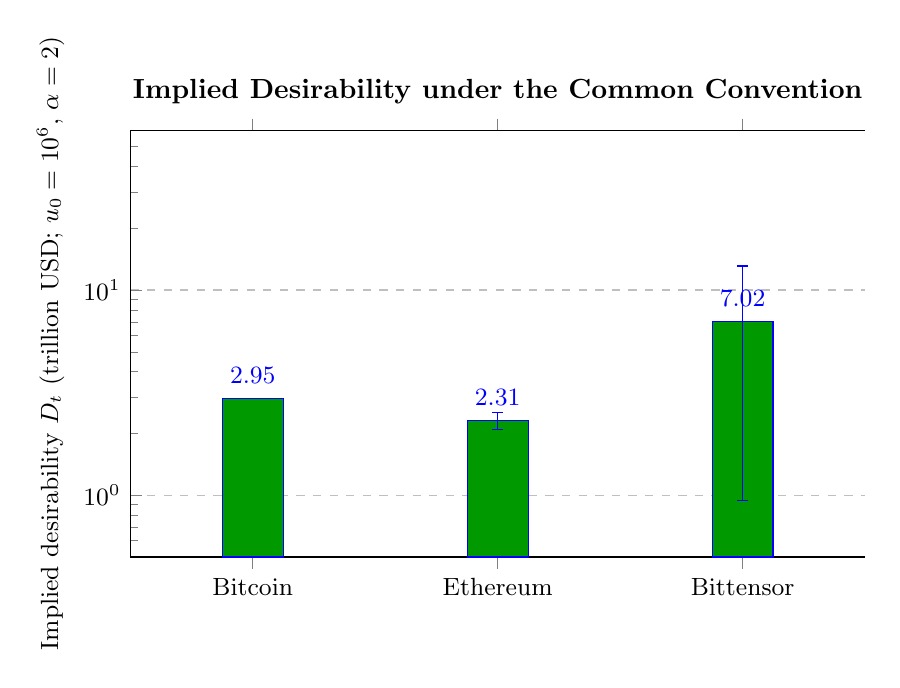
\begin{tikzpicture}
\begin{axis}[
    ybar,
    bar width=22pt,
    ymode=log,
    log origin=infty,
    ymin=0.5, ymax=60,
    width=0.9\textwidth,
    height=7cm,
    enlarge x limits=0.25,
    ylabel={Implied desirability \( D_t \) (trillion USD; \( u_0 = 10^6 \), \( \alpha = 2 \))},
    symbolic x coords={Bitcoin, Ethereum, Bittensor},
    xtick=data,
    point meta=rawy,
    nodes near coords={\pgfmathprintnumber[fixed, precision=2]{\pgfplotspointmeta}},
    nodes near coords align={vertical},
    title={\textbf{Implied Desirability under the Common Convention}},
    ylabel style={font=\small},
    tick label style={font=\small},
    axis y line*=left,
    every node near coord/.append style={font=\small, yshift=2pt},
    ymajorgrids=true,
    grid style=dashed
]
\addplot+[
    fill=green!60!black,
    error bars/.cd,
    y dir=both,
    y explicit
] coordinates {
    (Bitcoin, 2.95) +- (0.0, 0.0)       % alpha-invariant (u-tilde = 1 by construction)
    (Ethereum, 2.31) +- (0.25, 0.22)    % alpha in [1.8, 2.2]: 2.09 to 2.56
    (Bittensor, 7.02) +- (26.95, 6.08)  % user range 15k-90k at alpha=2: 0.94 to 33.97
};
\end{axis}
\end{tikzpicture}
\caption{Implied desirability (log scale) under the common convention (\( u_0 = 10^6 \), \( \alpha = 2 \), \( \beta = 1.5 \)). Whiskers: for Ethereum, sensitivity to \( \alpha \in [1.8, 2.2] \); for Bittensor, the native user-count range (15{,}000--90{,}000) at baseline \(\alpha\). Bitcoin has \( \tilde{u} = 1 \) and is \(\alpha\)-invariant by construction. Full grids in Appendix~\ref{appendix:alpha_sensitivity}.}
\label{fig:desirability_scores_sensitivity}
\end{figure}




%%%%%%%%%%%%%%%%%%%%%%%%%%%%%%%%%%
\section{Conclusion}
This paper has developed a structural valuation framework in which \emph{economic scarcity}, the monetizable intersection of desirability and constrained access, is the foundational source of value for blockchain networks and, conceptually, for monetizable assets more broadly. The framework's five-element structure (Purpose, Incentives, Consensus, Tokenomics, Network Effects) maps protocol architecture onto the preconditions of value, and its attribution method recovers an \emph{implied desirability}, the residual of market valuation unexplained by measured scarcity and adoption under a disclosed convention. Applied to Bitcoin, Ethereum, and Bittensor as illustrations, the method yields a sharp and interpretable pattern: the two mature networks carry nearly identical implied desirability per normalized user, their valuations largely explained by measured structure, while the young network's valuation is dominated by the residual, i.e., by expectations of future utility and adoption rather than demonstrated present-day fundamentals.

The framework's principal limitations define its research agenda. Implied desirability is an attribution, not an identified structural estimate: it absorbs expectations, liquidity, and measurement error alongside protocol utility, and separating these components requires independent measurements or identifying restrictions. The mapping from network usefulness to native-token value capture (velocity, fee flows, holding requirements) is summarized within Tokenomics rather than modeled, and the three-protocol illustration does not establish generality across asset classes. Extending the framework dynamically, in the direction of \citet{cong2021tokenomics}, validating the desirability residual against independent panels of fee revenue and developer activity, and applying the structural lens to decentralized AI, data networks, and tokenized real-world assets are the natural next steps.


%%%%%%%%%%%%%%%%%%%%%%%%%%%%%%%%%%%%%%%%%%%%%%%%%%%%%%%%

\section*{Data Availability Statement}
The data and code that support the findings of this study are openly available in Zenodo at \url{https://doi.org/10.5281/zenodo.24051776} and in GitHub at \url{https://github.com/apapadogiannis/economic-scarcity-as-value}. The archive contains the date-stamped input values with per-cell sources, the computational pipeline that regenerates every table and figure in Section~5 and Appendix~\ref{appendix:alpha_sensitivity}, and an automated test suite. All input values were derived from the following resources available in the public domain, as recorded in the archive: CoinGecko (market capitalizations), StakingRewards.com (annualized issuance rates), Glassnode (active addresses), Taostats and the Yuma \emph{State of Bittensor} reports (Bittensor participation and wallet counts), and Etherscan and BitInfoCharts (cumulative address counts).

\section*{Funding}
The author received no specific funding for this work.

\section*{Conflict of Interest}
The author declares no conflict of interest.

\section*{Author Contributions}
Agisilaos Papadogiannis: Conceptualization; Methodology; Software; Validation; Formal analysis; Investigation; Data curation; Writing (original draft); Writing (review and editing); Visualization.

\section*{Disclaimer}
This research was conducted independently and without funding, review, or endorsement. The views expressed are solely those of the author and do not represent any institutional position. This paper is for informational and academic purposes only and does not constitute financial, investment, tax, or legal advice, nor a recommendation to buy or sell any financial instrument. Any illustrative data used are from publicly available sources.

% Bibliography inlined (single-file manuscript; generated by BibTeX/apalike from the corrected references)
\begin{thebibliography}{}

\bibitem[Akerlof and Kranton, 2010]{akerlof2010identity}
Akerlof, G.~A. and Kranton, R.~E. (2010).
\newblock {\em Identity Economics: How Our Identities Shape Our Work, Wages,
  and Well-Being}.
\newblock Princeton University Press.

\bibitem[Bakhtiar et~al., 2023]{bakhtiar2023network}
Bakhtiar, T., Luo, X., and Adelopo, I. (2023).
\newblock Network effects and store-of-value features in the cryptocurrency
  market.
\newblock {\em Technology in Society}, 74:102320.

\bibitem[Barberis et~al., 1998]{barberis1998investor}
Barberis, N., Shleifer, A., and Vishny, R. (1998).
\newblock A model of investor sentiment.
\newblock {\em Journal of Financial Economics}, 49(3):307--343.

\bibitem[Barberis et~al., 2005]{barberis2005comovement}
Barberis, N., Shleifer, A., and Wurgler, J. (2005).
\newblock Comovement.
\newblock {\em Journal of Financial Economics}, 75(2):283--317.

\bibitem[Barney, 1991]{barney1991firm}
Barney, J. (1991).
\newblock Firm resources and sustained competitive advantage.
\newblock {\em Journal of Management}, 17(1):99--120.

\bibitem[Benartzi and Thaler, 1995]{benartzi1995myopic}
Benartzi, S. and Thaler, R.~H. (1995).
\newblock Myopic loss aversion and the equity premium puzzle.
\newblock {\em Quarterly Journal of Economics}, 110(1):73--92.

\bibitem[Benedetti and Rodriguez-Garnica, 2021]{benedetti2021tokenized}
Benedetti, H. and Rodriguez-Garnica, G. (2021).
\newblock Tokenized assets and securities.
\newblock {\em SSRN Electronic Journal}.
\newblock Available at SSRN: \url{https://ssrn.com/abstract=4101392}.

\bibitem[Benet, 2014]{benet2014ipfs}
Benet, J. (2014).
\newblock {IPFS - Content Addressed, Versioned, P2P File System}.
\newblock \url{https://arxiv.org/abs/1407.3561}.
\newblock arXiv:1407.3561 [cs.NI].

\bibitem[Biais et~al., 2020]{biais2020blockchain}
Biais, B., Bisi{\`e}re, C., Bouvard, M., and Casamatta, C. (2020).
\newblock The blockchain folk theorem.
\newblock {\em The Review of Financial Studies}, 33(1):171--203.

\bibitem[{BitInfoCharts}, 2025]{bitinfochartsBTC}
{BitInfoCharts} (2025).
\newblock Bitcoin number of unique addresses.
\newblock Accessed August 2025.
\newblock
  \url{https://bitinfocharts.com/comparison/bitcoin-uniqueaddresses.html}.

\bibitem[{Bittensor Documentation}, 2026]{yuma2025yuma}
{Bittensor Documentation} (2026).
\newblock Yuma Consensus.
\newblock \url{https://www.bittensor.com/docs/internals/consensus}.
\newblock Accessed November 2026.

\bibitem[Bonneau et~al., 2015]{bonneau2015sok}
Bonneau, J., Miller, A., Clark, J., Narayanan, A., Kroll, J.~A., and Felten,
  E.~W. (2015).
\newblock SoK: Research perspectives and challenges for Bitcoin and
  cryptocurrencies.
\newblock {\em IEEE Symposium on Security and Privacy}, pages 104--121.

\bibitem[Bouteska et~al., 2024]{bouteska2024cryptocurrency}
Bouteska, A., Abedin, M.~Z., Hajek, P., and Yuan, K. (2024).
\newblock Cryptocurrency price forecasting: A comparative analysis of ensemble
  learning and deep learning methods.
\newblock {\em International Review of Financial Analysis}, 92:103055.

\bibitem[Brealey et~al., 2022]{brealey2022principles}
Brealey, R.~A., Myers, S.~C., and Allen, F. (2022).
\newblock {\em Principles of Corporate Finance}.
\newblock McGraw-Hill Education, 14 edition.

\bibitem[Briscoe et~al., 2006]{briscoe2006metcalfe}
Briscoe, B., Odlyzko, A., and Tilly, B. (2006).
\newblock Metcalfe's law is wrong.
\newblock {\em IEEE Spectrum}, 43(7):34--39.

\bibitem[Brousseau and Curien, 2007]{brousseau2007internet}
Brousseau, E. and Curien, N. (2007).
\newblock {\em Internet and Digital Economics: Principles and Methods}.
\newblock Cambridge University Press.

\bibitem[Buterin, 2014]{buterin2014ethereum}
Buterin, V. (2014).
\newblock Ethereum: A next-generation smart contract and decentralized
  application platform.
\newblock \url{https://ethereum.org/en/whitepaper/}.
\newblock Accessed August 2025.

\bibitem[Buterin, 2022]{buterin2022proof}
Buterin, V. (2022).
\newblock {\em Proof of Stake: The Making of Ethereum and the Philosophy of
  Blockchains}.
\newblock Seven Stories Press, New York.

\bibitem[Campbell et~al., 1997]{campbell1997econometrics}
Campbell, J.~Y., Lo, A.~W., and MacKinlay, A.~C. (1997).
\newblock {\em The Econometrics of Financial Markets}.
\newblock Princeton University Press.

\bibitem[Canidio et~al., 2021]{canidio2021tokens}
Canidio, A., Danos, V., Marcassa, S., and Prat, J. (2021).
\newblock Tokens and ICOs: A review of the economic literature.
\newblock In {\em Principles of Blockchain Systems}, Synthesis Lectures on
  Computer Science. Springer.
\newblock \url{https://doi.org/10.1007/978-3-031-01807-7_8}.

\bibitem[Caringella et~al., 2024]{caringella2024bach}
Caringella, M., Violante, F., De~Lucci, F., Galantucci, S., and Costantini,
  M.~B. (2024).
\newblock BACH: A tool for analyzing blockchain transactions using address
  clustering heuristics.
\newblock {\em Information}, 15(10):589.

\bibitem[Catalini and Gans, 2020]{catalini2020some}
Catalini, C. and Gans, J.~S. (2020).
\newblock Some simple economics of the blockchain.
\newblock {\em Communications of the ACM}, 63(7):80--90.

\bibitem[Caves et~al., 1983]{caves1983contractual}
Caves, R.~E., Crookell, H., and Killing, J.~P. (1983).
\newblock Contractual arrangements in international technology transfer.
\newblock {\em Journal of International Business Studies}, 14(2):1--24.

\bibitem[Cong and He, 2019]{cong2019blockchain}
Cong, L.~W. and He, Z. (2019).
\newblock Blockchain disruption and smart contracts.
\newblock {\em The Review of Financial Studies}, 32(5):1754--1797.

\bibitem[Cong et~al., 2021]{cong2021tokenomics}
Cong, L.~W., Li, Y., and Wang, N. (2021).
\newblock Tokenomics: Dynamic adoption and valuation.
\newblock {\em The Review of Financial Studies}, 34(3):1105--1155.

\bibitem[Conley, 2017]{conley2021blockchain}
Conley, J.~P. (2017).
\newblock Blockchain and the economics of crypto-tokens and initial coin
  offerings.
\newblock Vanderbilt University Department of Economics Working Paper
  VUECON-17-00008.

\bibitem[Damodaran, 2012]{damodaran2012investment}
Damodaran, A. (2012).
\newblock {\em Investment Valuation: Tools and Techniques for Determining the
  Value of Any Asset}.
\newblock Wiley, 3 edition.

\bibitem[Daniel et~al., 1998]{daniel1998investor}
Daniel, K., Hirshleifer, D., and Subrahmanyam, A. (1998).
\newblock Investor psychology and security market under- and overreactions.
\newblock {\em Journal of Finance}, 53(6):1839--1885.

\bibitem[Demsetz, 1973]{demsetz1973industry}
Demsetz, H. (1973).
\newblock Industry structure, market rivalry, and public policy.
\newblock {\em Journal of Law and Economics}, 16(1):1--9.

\bibitem[Diniz-Maganini et~al., 2021]{dinizmaganini2021bitcoin}
Diniz-Maganini, N., Diniz, E.~H., and Rasheed, A.~A. (2021).
\newblock Bitcoin’s price efficiency and safe haven properties during the
  COVID-19 pandemic: A comparison.
\newblock {\em Research in International Business and Finance}, 58:101472.

\bibitem[Easley and Kleinberg, 2010]{easley2010networks}
Easley, D. and Kleinberg, J. (2010).
\newblock {\em Networks, Crowds, and Markets: Reasoning About a Highly
  Connected World}.
\newblock Cambridge University Press.

\bibitem[Easley et~al., 2019]{easley2019from}
Easley, D., O'Hara, M., and Basu, S. (2019).
\newblock From mining to markets: The evolution of Bitcoin transaction fees.
\newblock {\em Journal of Financial Economics}, 134(1):91--109.

\bibitem[Easterbrook and Fischel, 1984]{easterbrook1984close}
Easterbrook, F.~H. and Fischel, D.~R. (1984).
\newblock Close corporations and agency costs.
\newblock {\em Stanford Law Review}, 38(2):271--301.

\bibitem[{Ethereum Foundation}, 2023]{ethereumSupplyFAQ}
{Ethereum Foundation} (2023).
\newblock Components of ETH issuance.
\newblock
  \url{https://ethereum.org/en/roadmap/merge/issuance/#components-of-eth-issuance}.

\bibitem[{Etherscan}, 2025]{etherscan}
{Etherscan} (2025).
\newblock Ethereum unique addresses chart.
\newblock Accessed August 2025.

\bibitem[Evans, 2003a]{evans2003two}
Evans, D.~S. (2003a).
\newblock The antitrust economics of two-sided markets.
\newblock {\em Yale Journal on Regulation}, 20(2):325--381.

\bibitem[Evans, 2003b]{evans2003platform}
Evans, D.~S. (2003b).
\newblock Some empirical aspects of multi-sided platform industries.
\newblock {\em Review of Network Economics}, 2(3):191--209.

\bibitem[Gallini, 2002]{gallini2002intellectual}
Gallini, N.~T. (2002).
\newblock The economics of patents: Lessons from recent U.S. patent reform.
\newblock {\em Journal of Economic Perspectives}, 16(2):131--154.

\bibitem[Gandal and Halaburda, 2016]{GandalHalaburda2016}
Gandal, N. and Halaburda, H. (2016).
\newblock Can we predict the winner in a market with network effects?
  Competition in cryptocurrency market.
\newblock {\em Games}, 7(3):1--21.

\bibitem[Gangwal et~al., 2023]{gangwal2023survey}
Gangwal, A., Gangavalli, H.~R., and Thirupathi, A. (2023).
\newblock A survey of layer-two blockchain protocols.
\newblock {\em Journal of Network and Computer Applications}, 209:103539.

\bibitem[Gans, 2019]{gans2019economics}
Gans, J.~S. (2019).
\newblock The fine print in smart contracts.
\newblock National Bureau of Economic Research Working Paper No. 25443.
\newblock \url{https://doi.org/10.3386/w25443}.

\bibitem[{Glassnode}, 2025a]{glassnodeBTC}
{Glassnode} (2025a).
\newblock Bitcoin: Total and active address metrics.
\newblock Accessed August 5, 2025.
\newblock \url{https://studio.glassnode.com/charts/addresses.Count?a=BTC}.

\bibitem[{Glassnode}, 2025b]{glassnodeETH}
{Glassnode} (2025b).
\newblock Ethereum: Total and active address metrics.
\newblock Accessed August 5, 2025.
\newblock \url{https://studio.glassnode.com/charts/addresses.Count?a=ETH}.

\bibitem[Gregory and Mini, 2025]{gregory2025token}
Gregory, R. and Mini, T. (2025).
\newblock Token economics.
\newblock In Beck, R., editor, {\em Elgar Encyclopedia of Cryptocurrencies,
  Blockchain, and DLT}. Edward Elgar.
\newblock University of Miami Business School Research Paper No. 5136771.

\bibitem[Hansmann, 1996]{hansmann2001ownership}
Hansmann, H. (1996).
\newblock {\em The Ownership of Enterprise}.
\newblock Harvard University Press.

\bibitem[Hassan et~al., 2025]{hassan2025web3}
Hassan, M.~A., Jamshidi, M.~B., Manh, B.~D., Chu, N.~H., Nguyen, C.-H., Hieu,
  N.~Q., Nguyen, C.~T., Hoang, D.~T., Nguyen, D.~N., Huynh, N.~V., et~al.
  (2025).
\newblock Enabling technologies for Web 3.0: A comprehensive survey.
\newblock {\em Computer Networks}, 264:111242.

\bibitem[Hayes, 2015]{hayes2015cost}
Hayes, A.~S. (2015).
\newblock A cost of production model for Bitcoin.
\newblock {\em SSRN Electronic Journal}.

\bibitem[He et~al., 2022]{he2022address}
He, X., He, K., Lin, S., Yang, J., and Mao, H. (2022).
\newblock Bitcoin address clustering method based on multiple heuristic
  conditions.
\newblock {\em IET Blockchain}, 2(2):44--56.

\bibitem[Hong et~al., 2000]{hong2000bad}
Hong, H., Lim, T., and Stein, J.~C. (2000).
\newblock Bad news travels slowly: Size, analyst coverage, and the
  profitability of momentum strategies.
\newblock {\em Journal of Finance}, 55(1):265--295.

\bibitem[Hong and Stein, 2007]{hong2007disagreement}
Hong, H. and Stein, J.~C. (2007).
\newblock Disagreement and the stock market.
\newblock {\em Journal of Economic Perspectives}, 21(2):109--128.

\bibitem[Hotelling, 1931]{hotelling1931economics}
Hotelling, H. (1931).
\newblock The economics of exhaustible resources.
\newblock {\em Journal of Political Economy}, 39(2):137--175.

\bibitem[Huberman et~al., 2022]{huberman2021monetizing}
Huberman, G., Leshno, J., and Moallemi, C. (2022).
\newblock Monetizing blockchain: Insights from Bitcoin.
\newblock {\em Journal of Financial Economics}, 144(1):147--174.

\bibitem[Jaffe et~al., 1993]{jaffe1993geographic}
Jaffe, A.~B., Trajtenberg, M., and Henderson, R. (1993).
\newblock Geographic localization of knowledge spillovers as evidenced by
  patent citations.
\newblock {\em Quarterly Journal of Economics}, 108(3):577--598.

\bibitem[Jevons, 1871]{jevons1871political}
Jevons, W.~S. (1871).
\newblock {\em The Theory of Political Economy}.
\newblock Macmillan.

\bibitem[Kilian, 2009]{kilian2009oil}
Kilian, L. (2009).
\newblock Oil price shocks, monetary policy and stagflation.
\newblock In Fry, R., Jones, C., and Kent, C., editors, {\em Inflation in an
  Era of Relative Price Shocks}, RBA Annual Conference Volume. Reserve Bank of
  Australia.

\bibitem[Klages-Mundt et~al., 2020]{klages2020stablecoins2}
Klages-Mundt, A., Harz, D., Gudgeon, L., Liu, J., and Minca, A. (2020).
\newblock Stablecoins 2.0: Economic foundations and risk-based models.
\newblock In {\em Proceedings of the 2nd ACM Conference on Advances in
  Financial Technologies (AFT ’20)}, pages 59--79.

\bibitem[Koutmos, 2018]{Koutmos2018}
Koutmos, D. (2018).
\newblock Bitcoin returns and transaction activity.
\newblock {\em Economics Letters}, 167:81--85.

\bibitem[Kraakman et~al., 2017]{kraakman2017anatomy}
Kraakman, R., Armour, J., Davies, P., Enriques, L., Hansmann, H., Hertig, G.,
  Hopt, K.~J., Kanda, H., and Rock, E.~B. (2017).
\newblock {\em The Anatomy of Corporate Law: A Comparative and Functional
  Approach}.
\newblock Oxford University Press.

\bibitem[Kristoufek, 2015]{Kristoufek2015}
Kristoufek, L. (2015).
\newblock What are the main drivers of the Bitcoin price? Evidence from wavelet
  coherence analysis.
\newblock {\em PLoS ONE}, 10(4):e0123923.

\bibitem[Lee et~al., 2020]{lee2020measurements}
Lee, X.~T., Khan, A., Gupta, S.~S., Ong, Y.~H., and Liu, X. (2020).
\newblock Measurements, analyses, and insights on the entire Ethereum
  blockchain network.
\newblock In {\em Proceedings of The Web Conference 2020}, pages 155--166,
  Taipei, Taiwan. ACM.

\bibitem[Lin, 2025]{lin2025culture}
Lin, Z.-Y. (2025).
\newblock The effect of culture on global NFT investor attention.
\newblock {\em Pacific-Basin Finance Journal}, 90:102696.

\bibitem[Liu et~al., 2022]{LiuTsyvinski2022}
Liu, Y., Tsyvinski, A., and Wu, X. (2022).
\newblock Common risk factors in cryptocurrency.
\newblock {\em The Journal of Finance}, 77(2):1133--1177.

\bibitem[Lu et~al., 2025]{lu2025unveiling}
Lu, H., Luo, X.~R., Ma, S.~S., and Chen, R. (2025).
\newblock Unveiling the paradox of NFT digital scarcity: Impacts of digital
  scarcity on online trading and social behaviors.
\newblock {\em Information \& Management}, 62(7):104205.

\bibitem[Menger, 1871]{menger1871principles}
Menger, C. (1871).
\newblock {\em Principles of Economics}.
\newblock Ludwig von Mises Institute.

\bibitem[Merton, 1987]{merton1987simple}
Merton, R.~C. (1987).
\newblock A simple model of capital market equilibrium with incomplete
  information.
\newblock {\em The Journal of Finance}, 42(3):483--510.

\bibitem[Metcalfe, 1995]{metcalfe1995metcalfe}
Metcalfe, R.~M. (1995).
\newblock Metcalfe's law: A network becomes more valuable as it reaches more
  users.
\newblock {\em InfoWorld}, 17(40):53.

\bibitem[Modigliani and Miller, 1961]{modigliani1961dividend}
Modigliani, F. and Miller, M.~H. (1961).
\newblock Dividend policy, growth, and the valuation of shares.
\newblock {\em Journal of Business}, 34(4):411--433.

\bibitem[Murphy, 1999]{murphy1999executive}
Murphy, K.~J. (1999).
\newblock Executive compensation.
\newblock {\em Handbook of Labor Economics}, 3:2485--2563.

\bibitem[Nadler and Guo, 2020]{nadler2020fair}
Nadler, P. and Guo, Y. (2020).
\newblock The fair value of a token: How do markets price cryptocurrencies?
\newblock {\em Research in International Business and Finance}, 52:101108.

\bibitem[Nakamoto, 2008]{nakamoto2008bitcoin}
Nakamoto, S. (2008).
\newblock Bitcoin: A peer-to-peer electronic cash system.
\newblock \url{https://bitcoin.org/bitcoin.pdf}.

\bibitem[{OpenTensor Foundation}, 2023]{opentensor2023taoeconomy}
{OpenTensor Foundation} (2023).
\newblock TAO token economy explained.
\newblock
  \url{https://blog.bittensor.com/tao-token-economy-explained-17a3a90cd44e}.
\newblock Accessed August 5, 2025.

\bibitem[{OpenTensor Foundation}, 2026]{opentensor_governance}
{OpenTensor Foundation} (2026).
\newblock Governance.
\newblock \url{https://www.bittensor.com/docs/guides/governance}.
\newblock Accessed November 2026.

\bibitem[Paech, 2017]{paech2017governance}
Paech, P. (2017).
\newblock The governance of blockchain financial networks.
\newblock {\em Modern Law Review}, 80(6):1073--1110.

\bibitem[Pagano and Röell, 1998]{pagano1998choice}
Pagano, M. and Röell, A. (1998).
\newblock The choice of stock ownership structure: agency costs, monitoring,
  and the decision to go public.
\newblock {\em The Quarterly Journal of Economics}, 113(1):187--225.

\bibitem[Papadogiannis, 2026a]{papadogiannis2025dualrisk}
Papadogiannis, A. (2026a).
\newblock From unified discounting to dual-risk: A new lens on DCF valuation.
\newblock {\em Finance Research Open}, 2(1):100096.
\newblock \url{https://doi.org/10.1016/j.finr.2026.100096}.

\bibitem[Papadogiannis, 2026b]{papadogiannis2025scarcity}
Papadogiannis, A. (2026b).
\newblock Valuing scarcity: A general framework for Bitcoin, gold, and
  traditional assets.
\newblock {\em Financial Economics Letters}, 5(2):1--18.
\newblock \url{https://doi.org/10.58567/fel05020001}.

\bibitem[Parker et~al., 2016]{parker2016platform}
Parker, G., Van~Alstyne, M., and Choudary, S.~P. (2016).
\newblock {\em Platform Revolution: How Networked Markets Are Transforming the
  Economy}.
\newblock W. W. Norton \& Company.

\bibitem[Peterson, 2018]{Peterson2018}
Peterson, T. (2018).
\newblock Metcalfe's law as a model for Bitcoin's value.
\newblock {\em Alternative Investment Analyst Review}, 7(2):9--18.

\bibitem[Pontiff, 2006]{pontiff2006liquidity}
Pontiff, J. (2006).
\newblock Costly arbitrage and the myth of idiosyncratic risk.
\newblock {\em Journal of Accounting and Economics}, 42(1--2):35--52.

\bibitem[Porter, 1985]{porter1985competitive}
Porter, M.~E. (1985).
\newblock {\em Competitive Advantage: Creating and Sustaining Superior
  Performance}.
\newblock Free Press.

\bibitem[Ramachandran et~al., 2021]{ramachandran2021defi}
Ramachandran, A., Harvey, C.~R., and Santoro, J. (2021).
\newblock {\em DeFi and the Future of Finance}.
\newblock Wiley, Hoboken, NJ.

\bibitem[Rao, 2023]{rao2023bittensor}
Rao, Y. (2023).
\newblock Bittensor: A decentralized intelligence market.
\newblock \url{https://bittensor.com/whitepaper}.

\bibitem[Rao et~al., 2020]{rao2020bittensor}
Rao, Y., Steeves, J., Shaabana, A., Attevelt, D., and McAteer, M. (2020).
\newblock Bittensor: A peer-to-peer intelligence market.
\newblock arXiv preprint arXiv:2003.03917.
\newblock \url{https://arxiv.org/abs/2003.03917}.

\bibitem[Reed, 2001]{reed2001law}
Reed, D.~P. (2001).
\newblock The law of the pack.
\newblock {\em Harvard Business Review}, 79(2):23--24.

\bibitem[Rochet and Tirole, 2003]{rochet2003platform}
Rochet, J.-C. and Tirole, J. (2003).
\newblock Platform competition in two-sided markets.
\newblock {\em Journal of the European Economic Association}, 1(4):990--1029.

\bibitem[Rochet and Tirole, 2006]{rochet2006two}
Rochet, J.-C. and Tirole, J. (2006).
\newblock Two-sided markets: A progress report.
\newblock {\em RAND Journal of Economics}, 37(3):645--667.

\bibitem[Saleh, 2021]{saleh2021blockchain}
Saleh, F. (2021).
\newblock Blockchain without waste: Proof-of-Stake.
\newblock {\em The Review of Financial Studies}, 34(3):1156--1190.

\bibitem[Schär, 2021]{schar2021defi}
Schär, F. (2021).
\newblock Decentralized finance: On blockchain- and smart contract-based
  financial markets.
\newblock {\em Federal Reserve Bank of St. Louis Review}, 103(2):153--174.

\bibitem[Shapiro, 1985]{shapiro1985licensing}
Shapiro, C. (1985).
\newblock Patent licensing and R\&D rivalry.
\newblock {\em The American Economic Review}, 75(2):25--30.
\newblock Papers and Proceedings of the Ninety-Seventh Annual Meeting of the
  American Economic Association.

\bibitem[Shleifer and Vishny, 1997]{shleifer1997survey}
Shleifer, A. and Vishny, R.~W. (1997).
\newblock A survey of corporate governance.
\newblock {\em Journal of Finance}, 52(2):737--783.

\bibitem[Singh, 2025]{singh2025blockchain}
Singh, A.~P. (2025).
\newblock Blockchain technology: Core mechanisms, evolution, and future
  implementation challenges.
\newblock \url{https://arxiv.org/abs/2505.08772}.
\newblock arXiv:2505.08772v1, National Institute of Technology,
  Tiruchirappalli.

\bibitem[Singh et~al., 2024]{singh2023blockchain}
Singh, S., Gaur, A., and Singh, D. (2024).
\newblock Blockchain-based governance: Implications for organizational
  boundaries and structures.
\newblock {\em British Journal of Management}, 35(4):1692--1699.
\newblock First published online: December 4, 2023.

\bibitem[{Staking Rewards}, 2025]{stakingrewards2025eth}
{Staking Rewards} (2025).
\newblock Ethereum staking yields and inflation (2025).
\newblock \url{https://www.stakingrewards.com/earn/ethereum/}.
\newblock Accessed August 2025.

\bibitem[Stigler, 1971]{stigler1971regulation}
Stigler, G.~J. (1971).
\newblock The theory of economic regulation.
\newblock {\em The Bell Journal of Economics and Management Science},
  2(1):3--21.

\bibitem[{Taostats}, 2025]{taostats_accounts}
{Taostats} (2025).
\newblock Bittensor number of accounts.
\newblock Accessed August 5, 2025.
\newblock \url{https://taostats.io/accounts}.

\bibitem[Thaler and Johnson, 1997]{thaler1997effect}
Thaler, R.~H. and Johnson, E.~J. (1997).
\newblock The effect of myopia and loss aversion on risk taking: An
  experimental test.
\newblock {\em Quarterly Journal of Economics}, 112(2):647--661.

\bibitem[Tirole, 1988]{tirole1988theory}
Tirole, J. (1988).
\newblock {\em The Theory of Industrial Organization}.
\newblock MIT Press.

\bibitem[{Ultrasound Money}, 2025]{eip1559stats}
{Ultrasound Money} (2025).
\newblock Ethereum supply and burn statistics.
\newblock \url{https://ultrasound.money}.
\newblock Accessed August 5, 2025.

\bibitem[Urquhart, 2022]{urquhart2022ethereum}
Urquhart, A. (2022).
\newblock Under the hood of the Ethereum blockchain.
\newblock {\em Finance Research Letters}, 47:102628.

\bibitem[Urquhart and Yarovaya, 2023]{urquhart2023future}
Urquhart, A. and Yarovaya, L. (2023).
\newblock Cryptocurrency research: Future directions.
\newblock {\em The European Journal of Finance}.

\bibitem[Varian, 1992]{varian1992microeconomic}
Varian, H.~R. (1992).
\newblock {\em Microeconomic Analysis}.
\newblock W. W. Norton \& Company.

\bibitem[Victor, 2018]{victor2018ethereum}
Victor, F. (2018).
\newblock Address clustering heuristics for Ethereum.
\newblock In {\em 2018 IEEE International Conference on Blockchain and
  Cryptocurrency (ICBC)}, pages 1--7.

\bibitem[Williams, 1938]{williams1938theory}
Williams, J.~B. (1938).
\newblock {\em The Theory of Investment Value}.
\newblock Harvard University Press.

\bibitem[Yermack, 2017]{yermack2017corporate}
Yermack, D. (2017).
\newblock Corporate governance and blockchains.
\newblock {\em Review of Finance}, 21(1):7--31.

\bibitem[Zhang et~al., 2010]{zhang2010value}
Zhang, J., Wedel, M., and Pieters, R. (2010).
\newblock The value of it-enabled retailer learning: Personalized product
  recommendations and customer store loyalty in online retailing.
\newblock {\em Information Systems Research}, 21(3):416--431.

\end{thebibliography}

%%%%%%%%%%%%%%%%%%%%%%%%%%%%%%%%%%%%%
\clearpage
\appendix
\section{Candidates for the Interaction Function \( F(D_t, S_t) \)}
\label{appendix:f_forms}

The interaction function \( F(D_t, S_t) \) captures how desirability and physical scarcity reinforce one another to generate economic scarcity. While the main text leaves \( F \) general, several functional forms may be considered depending on empirical context, interpretive goals, or analytical tractability.

\paragraph{A.1 Separable Power Form.}  
\begin{equation}
F(D_t, S_t) = (D_t)^\beta \cdot (S_t)^\gamma,
\tag{A.1}
\end{equation}
where \( \beta, \gamma > 0 \). This form assumes independent, nonlinear reinforcement from each component. It preserves symmetry when \( \beta = \gamma \), and supports log-linear estimation:
\[
\log(\text{Economic Scarcity}_t) = (1+\beta) \log D_t + (1+\gamma) \log S_t.
\]

\paragraph{A.2 Additive Interaction Form.}  
\begin{equation}
F(D_t, S_t) = 1 + \lambda \cdot D_t \cdot S_t,
\tag{A.2}
\end{equation}
where \( \lambda > 0 \). This form captures first-order complementarity and ensures positive value even when either component is small. It is simple, intuitive, and useful for linear approximations in early-stage adoption or limited interaction settings.

\paragraph{A.3 Logarithmic Amplification Form.}  
\begin{equation}
F(D_t, S_t) = \log(1 + \lambda D_t S_t),
\tag{A.3}
\end{equation}
which introduces diminishing marginal amplification: the function is concave and sublinear in \( D_t S_t \), so that each increment of the product contributes less additional amplification than the last. It is, however, \emph{unbounded}, growing without limit (if slowly) as \( D_t S_t \to \infty \); it does not saturate at a finite ceiling. This form is suitable when marginal reinforcement weakens at scale, and it helps regularize functional behavior when the data range spans several orders of magnitude.

\paragraph{A.4 Network Effect Proxy.}  
\begin{equation}
F(D_t, S_t) \approx u_t^\alpha,
\tag{A.4}
\end{equation}
where \( u_t \) denotes the user base or adoption level, and \( \alpha \geq 1 \) reflects the strength of interaction effects. This form provides an empirical proxy for mutual reinforcement in scalable systems such as blockchain networks and digital platforms. It aligns with Metcalfe’s Law \citep{metcalfe1995metcalfe}, Reed’s Law \citep{reed2001law}, and modern platform economics \citep{evans2003two, rochet2006two, cong2019blockchain}.

Saturation in this case is conditional. Unlike concave forms such as the logarithmic specification above, \( u_t^\alpha \) grows super-linearly without damping as adoption increases. However, if desirability \( D_t \) or perceived scarcity \( S_t \) lag behind user growth, or if network quality deteriorates with scale, the marginal value of new users may decline. In such cases, real-world saturation can emerge even if the functional form does not impose it explicitly. Thus, this proxy is best used in conjunction with behavioral or structural constraints that capture adoption-quality dynamics.

\paragraph{A.5 Bottleneck Constraint Form.}  
\begin{equation}
F(D_t, S_t) = \min(D_t, S_t),
\tag{A.5}
\end{equation}
which reflects the idea that value is constrained by the weaker of the two inputs. This is appropriate in environments where either demand or supply can become the binding constraint. Note that this form falls \emph{outside} the class of smooth interaction functions to which Proposition~2 applies: it is non-differentiable at \( D_t = S_t \), and away from that locus its partial derivative with respect to the larger input is zero, so it satisfies only weak (not strict) monotonicity. It is included here as an interpretable non-smooth alternative suitable for mechanism design or resource allocation models, not as an instance of the smooth class analyzed in the main text.


\paragraph{Remarks}
Each form above embodies a different assumption about how desirability and scarcity interact. Table~\ref{tab:F_forms_summary} summarizes key properties across forms. The general scarcity valuation framework remains agnostic to any specific \( F \), but the choice of form can significantly influence comparative statics, estimation strategies, and theoretical interpretations.

\begin{table}[H]
\centering
\caption{Summary of Candidate Forms for \( F(D_t, S_t) \)}
\label{tab:F_forms_summary}
\renewcommand{\arraystretch}{1.4}
\begin{tabular}{@{}L{3.5cm}L{4.0cm}<{\raggedright}L{3.5cm}L{4.2cm}@{}}
\toprule
\rowcolor{gray!15}
\textbf{Functional Form} & \textbf{Interaction Type} & \textbf{Saturation Behavior} & \textbf{Best Applied In} \\
\midrule
Power (\( D^\beta S^\gamma \)) & Nonlinear, multiplicative & No & Structural estimation \\
Additive (\( 1 + \lambda D S \)) & First-order complementarity & No & Linear models or early-stage regimes \\
Log (\( \log(1 + \lambda D S) \)) & Concave, diminishing marginal amplification & No (unbounded, sublinear) & High-scale systems or regularization \\
Network proxy (\( u^\alpha \)) & Empirical interaction via scale & Conditional & Blockchain, platforms \\
Minimum (\( \min(D, S) \)) & Bottleneck constraint (non-smooth; outside Prop.~2 class) & Yes & Hard constraints, frictional systems \\
\bottomrule
\end{tabular}
\end{table}


%%%%%%%%%%%%%%%%%%%%%%%%%%%%%%%%%%%%%%%%%%%%%%%%%%%%%%%%%%%%%%%%%%%%
\newpage
\section{Tokens vs. Equity: Similarities and Contrasts}
\label{appendix:tokens_vs_equity}

This appendix expands on the comparison introduced in Section~\ref{sec:framework_elements} and Table~\ref{tab:five_elements_stock_vs_token_main}, providing both a structural and functional mapping between equity-based enterprises and blockchain protocol economies. Blockchain-based tokens are often compared to common equity shares, as both represent digital stakes in an organized economic endeavor \citep{paech2017governance, yermack2017corporate}. 

The core distinction lies in their underlying architectures. Stockholders own part of a centralized legal entity, whose operations and value creation are coordinated through formal management within a corporate structure \citep{easterbrook1984close, hansmann2001ownership}. Token holders, by contrast, participate in a decentralized protocol economy, where value emerges from distributed execution, cryptographic guarantees, and incentive alignment \citep{gans2019economics, singh2023blockchain, cong2021tokenomics, schar2021defi}. In equity markets, the architecture is institutional and legal \citep{kraakman2017anatomy}; in blockchain networks, it is computational and protocol-based \citep{saleh2021blockchain, biais2020blockchain}. 

Despite these differences in enforcement substrate, both systems implement the same five economic primitives introduced in Section~\ref{sec:framework_elements}, Purpose, Incentives, Consensus, Tokenomics, and Network Effects, but through fundamentally different mechanisms. The main text's Table~\ref{tab:five_elements_stock_vs_token_main} summarizes these contrasts at a structural level. Here, we extend the analysis by mapping practical economic tasks performed by blockchain protocols and the ways in which they operationalize the five elements.

From the perspective of the five-element framework, equity markets express these primitives through corporate missions, compensation structures, governance processes, capital structure, and marketing strategies \citep{barney1991firm, murphy1999executive, shleifer1997survey, modigliani1961dividend, parker2016platform}. In blockchain protocols, the same primitives are embedded directly into protocol logic, executed through consensus algorithms, and enforced by software rather than law \citep{nakamoto2008bitcoin, buterin2022proof, rao2023bittensor}.

While Table~\ref{tab:five_elements_stock_vs_token_main} addresses the structural level, 
Table~\ref{tab:blockchain_tasks} illustrates practical manifestations of these elements. 
It lists representative economic tasks that blockchain networks are engineered to perform, 
along with example protocols that operationalize these tasks.


\begin{table}[H]
\centering
\caption{\textbf{Decentralized Economic Tasks Performed by Blockchain Networks.} 
Representative blockchain use cases mapped to protocol examples, showing how tokenized systems operationalize the five value elements in practice.}
\label{tab:blockchain_tasks}
\renewcommand{\arraystretch}{1.4}
\begin{tabular}{@{}>{\raggedright\arraybackslash}p{5.2cm} >{\raggedright\arraybackslash}p{4.8cm} L{5.5cm}@{}}
\toprule
\rowcolor{gray!15}
\textbf{Task / Function} & \textbf{Example Protocols} & \textbf{Description} \\
\midrule
Transferring value (payments) & Bitcoin, Litecoin & Peer-to-peer digital currency with fixed supply \citep{nakamoto2008bitcoin, gans2019economics} \\
Executing smart contracts & Ethereum, Solana & General-purpose computation and programmable transactions \citep{buterin2022proof, cong2021tokenomics} \\
Stablecoin issuance and value anchoring & MakerDAO (DAI), USDC & Tokens pegged to fiat via collateral or custody systems \citep{klages2020stablecoins2, schar2021defi} \\
Lending, borrowing, and DeFi primitives & Aave, Compound, Uniswap & Decentralized financial services through open liquidity protocols \citep{schar2021defi} \\
Consensus-based validation and staking & Ethereum 2.0, Cosmos & Network participation and security through bonded capital \citep{saleh2021blockchain} \\
Decentralized storage and file retrieval & Filecoin, Arweave & Verifiable, incentive-aligned decentralized file storage \citep{catalini2020some} \\
Machine learning and model evaluation & Bittensor & Tokenized AI ecosystem with incentivized training and validation \citep{rao2023bittensor} \\
Off-chain computation and hosting & Akash, Celestia & Cloud infrastructure and modular data layers \citep{gangwal2023survey} \\
Digital identity and naming & ENS, BrightID, Proof of Humanity & Self-sovereign identity and human verification \citep{bonneau2015sok} \\
Decentralized content and social media & Lens Protocol, Farcaster & Token-based social interaction platforms \citep{singh2023blockchain} \\
\bottomrule
\end{tabular}
\end{table}

Unlike stockholders, token holders have no guaranteed claim on future cash flows or statutory protections. Their economic security rests instead on decentralization, consensus rules, and incentive alignment, which together aim to ensure predictable execution and resistance to arbitrary interference. Value derives from access to services, governance participation, influence over protocol evolution, and exposure to network growth. This marks a shift from \textit{ownership of a legal entity} to \textit{participation in a protocol economy}.

\paragraph{Tokenization of Equity.}
Tokenization of equity refers to representing traditional shares as blockchain-based tokens \citep{benedetti2021tokenized}. While this may improve settlement efficiency, transparency, and custody, it does not alter the underlying legal or economic structure. Tokenized shares remain securities governed by corporate law, with the same rights and obligations as their non-tokenized counterparts. Tokenization changes the implementation of certain elements (Consensus and Custody) but leaves Purpose, Incentives, and Tokenomics rooted in the corporate framework.

\paragraph{Tokenizing the Internet?}
Web 2.0 platforms extract value from user participation without granting native economic stakes or enforceable rights \citep{hassan2025web3}. Web 3.0, in contrast, embeds governance, incentives, and access rights directly into protocol architecture via tokens. In this setting, the token is not an auxiliary feature but the economic infrastructure of decentralized trust.

\begin{tcolorbox}[title=\textbf{Centralization vs. Decentralization}]
Sustainable digital systems require either centralized infrastructure with legal protection or decentralized infrastructure with protocol guarantees. In the latter, the token coordinates the five elements, Purpose, Incentives, Consensus, Tokenomics, and Network Effects, through code, making it the operational and economic core of the system. In effect, the token becomes both the governance object and the medium of value transfer, unifying the technical and economic layers.
\end{tcolorbox}

%%%%%%%%%%%%%%%%%%%%%%%%%%%%%%%%%%%%%%%%%%%
\newpage
\section{Sensitivity and Normalization Analyses for Implied Desirability}
\label{appendix:alpha_sensitivity}

This appendix reports the sensitivity of implied desirability \(D_t\) (Equation~\ref{eq:desirability_2}) to the network-effect exponent \(\alpha\), the Bittensor user-count range, an \( n \log n \) network-effect specification, and the user-normalization scale \( u_0 \). All inputs match the main text (5 August 2025; \( \beta = 1.5 \); \( u_0 = 10^6 \) unless stated), and every value is generated by the paper's reproduction pipeline.

\paragraph{C.1 Sensitivity to a common \(\alpha\).}
Table~\ref{tab:alpha_sensitivity} applies each \(\alpha\) \emph{uniformly to all three protocols}, at baseline user estimates. The direction of the effect depends on the normalized user count: for \( \tilde{u}_t < 1 \), a higher \(\alpha\) shrinks \( \tilde{u}_t^{\alpha} \) and thus \emph{raises} inferred \( D_t \); for \( \tilde{u}_t > 1 \) it would lower it. Bitcoin, with \( \tilde{u} = 1 \), is invariant to \(\alpha\) by construction and serves as the reference point of the convention. The qualitative conclusion of the main text, BTC and ETH closely comparable, TAO the expectation-dominated outlier, holds at every \(\alpha\).

\begin{table}[H]
\centering
\caption{\textbf{Sensitivity of \(D_t\) (trillion USD) to a Common \(\alpha\) (August 2025; \( u_0 = 10^6 \), \( \beta = 1.5 \), baseline users)}}
\label{tab:alpha_sensitivity}
\renewcommand{\arraystretch}{1.3}
\begin{tabular}{@{}lcccc@{}}
\toprule
\rowcolor{gray!15}
\textbf{Network} & \(\alpha = 1.8\) & \(\alpha = 2.0\) (baseline) & \(\alpha = 2.2\) & \(\alpha = 2.5\) \\
\midrule
Bitcoin (BTC)   & 2.95 & 2.95 & 2.95 & 2.95 \\
Ethereum (ETH)  & 2.09 & 2.31 & 2.56 & 2.98 \\
Bittensor (TAO) & 3.55 & 7.02 & 13.9 & 38.6 \\
\bottomrule
\end{tabular}
\end{table}

\paragraph{C.2 Bittensor user-count range.}
At the baseline convention (\(\alpha = 2\)), \( D_{\text{TAO}} \) equals \(34.0\), \(7.02\), and \(0.94\) trillion USD at \( u = 15{,}000 \), \( 33{,}000 \), and \( 90{,}000 \) respectively. Even at the most generous adoption estimate, TAO's implied desirability remains of the same order as Bitcoin's and Ethereum's despite a market capitalization three orders of magnitude smaller, so the main text's interpretation is not an artifact of the user-count choice.

\paragraph{C.3 \( n \log n \) specification.}
\citet{briscoe2006metcalfe} argue that network value scales as \( n \log n \) rather than quadratically. Replacing \( \tilde{u}_t^{\alpha} \) with \( \tilde{u}_t \log(1 + u_t) \) yields implied desirabilities of \(0.21\), \(0.10\), and \(0.022\) trillion USD for BTC, ETH, and TAO at baseline users (TAO range: \(0.0074\)--\(0.053\)). Levels change, as they must under a different convention, but the qualitative pattern is preserved: BTC and ETH remain within a small factor of each other, while TAO's residual per unit of adoption remains disproportionately large relative to its market capitalization.

\paragraph{C.4 Invariance to the normalization scale \( u_0 \).}
Under a rescaling \( u_0 \mapsto u_0 / c \), Equation~\eqref{eq:desirability_2} multiplies every \( D_t \) by \( c^{\alpha} \). With a \emph{common} \(\alpha\), the multiplication is uniform across protocols and the cross-protocol ordering of \( D_t \) is invariant to the choice of \( u_0 \); Table~\ref{tab:rescaling} demonstrates this numerically, and shows that with protocol-specific exponents (\(\alpha = 2\) for BTC/ETH, \(\alpha = 2.5\) for TAO) the ordering \emph{changes} with the unit convention. This dependence is why the baseline analysis uses one exponent for all networks.

\begin{table}[H]
\centering
\caption{\textbf{Cross-Protocol Ordering of \(D_t\) under Alternative Normalization Scales \(u_0\)}}
\label{tab:rescaling}
\renewcommand{\arraystretch}{1.3}
\begin{tabular}{@{}lccc@{}}
\toprule
\rowcolor{gray!15}
\textbf{Specification} & \(u_0 = 1\) & \(u_0 = 10^3\) & \(u_0 = 10^6\) \\
\midrule
Common \(\alpha = 2\) (baseline) & TAO $>$ BTC $>$ ETH & TAO $>$ BTC $>$ ETH & TAO $>$ BTC $>$ ETH \\
Mixed \(\alpha\) (2 / 2 / 2.5)   & BTC $>$ ETH $>$ TAO & BTC $>$ ETH $>$ TAO & TAO $>$ BTC $>$ ETH \\
\bottomrule
\end{tabular}

\vspace{0.4em}
\footnotesize
\textit{Note:} Under the common exponent the ordering is identical at every \(u_0\) (each \(D_t\) is rescaled by the same factor \(c^{\alpha}\)). Under mixed exponents the ordering depends on whether users are counted in raw units, thousands, or millions, i.e., it is an artifact of measurement units rather than an economic result.

\paragraph{C.5 Robustness to the component scores.}
Because the components \( C, E, B, G, R \) are expert assessments on the rubric of Table~\ref{tab:scoring_rubric}, we test whether the paper's cross-protocol conclusions depend on their precise values. Shifting any single score of any network by \( \pm 0.15 \) (thirty cases, clipped to \([0,1]\)) changes neither the ordering of \( S_t \) (BTC $>$ ETH $>$ TAO) nor the ordering of baseline implied desirability (TAO $>$ BTC $>$ ETH). Perturbing all fifteen scores simultaneously by independent uniform shocks on \([-0.15, 0.15]\) over 20{,}000 draws preserves the \( S_t \) ordering in 97.2\% of draws and the implied-desirability ordering in 100\%; the rare \( S_t \) reversals are BTC--ETH swaps requiring simultaneous adverse shifts of several Bitcoin scores. The qualitative conclusions are therefore not artifacts of the specific scores assigned.
\end{table}





\end{document}
